% =====================================================================
%  Cervical-cytology audit -- CVPR two-column preprint (camera-ready style)
%  Build: tectonic main.tex   (cvpr.sty inlines eso-pic; ieeenat_fullname bib)
% =====================================================================
\documentclass[10pt,twocolumn,letterpaper]{article}

\usepackage{cvpr}                 % CVPR two-column camera-ready style
\usepackage{microtype}
\usepackage{amsfonts}
\usepackage{pifont}               % \ding check / cross glyphs
\usepackage{dblfloatfix}          % robust placement of full-width (starred) floats
\graphicspath{{figures/}}
\setcounter{totalnumber}{12}

% float tuning (two-column aware) so full-width figures distribute, not pile up
\renewcommand{\topfraction}{0.92}\renewcommand{\bottomfraction}{0.70}
\renewcommand{\textfraction}{0.06}\renewcommand{\floatpagefraction}{0.78}
\renewcommand{\dbltopfraction}{0.92}\renewcommand{\dblfloatpagefraction}{0.78}

% hyperref last, then cleveref
\definecolor{linknavy}{rgb}{0.10,0.30,0.55}
\usepackage[pagebackref,breaklinks,colorlinks,allcolors=linknavy]{hyperref}
\usepackage[capitalize]{cleveref}

% ---- macros ----
\newcommand{\sipakmed}{\textsc{SIPaKMeD}\xspace}
\newcommand{\herlev}{\textsc{Herlev}\xspace}
\newcommand{\apacc}{\textsc{APACC}\xspace}
\newcommand{\hicervix}{\textsc{HiCervix}\xspace}
\newcommand{\pabn}{P(\mathrm{abn})}
\newcommand{\cmark}{\ding{51}}
\newcommand{\xmark}{\ding{55}}
\newcommand{\best}[1]{\textbf{#1}}   % highlight the winning value in a table/row
\DeclareMathOperator{\softmax}{softmax}

\def\confName{Preprint}
\def\confYear{2026}

\title{Internal Excellence, External Collapse: Auditing and Diagnosing a\\
Knowledge-Distilled Cervical Cytology Classifier Across Datasets}
\author{Anonymous\\ Preprint}

\begin{document}
\maketitle

\begin{abstract}
Cervical-cytology classifiers are routinely reported at near-ceiling \emph{single-dataset} accuracy
and presented as deployable screening tools. We show this number is a poor proxy for screening
readiness. We audit a knowledge-distilled classifier---an EfficientNet-B4 teacher (18.5\,M params)
distilled into an EfficientNet-B0 student (4.67\,M params)---trained on the five \sipakmed\
cytomorphology classes. In-distribution the student is genuinely excellent and, notably,
\emph{surpasses its own teacher} on every metric (accuracy $0.966$ vs.\ $0.943$, macro-$F_1$ $0.967$,
Cohen's $\kappa$ $0.958$, one-vs-rest AUROC $0.998$, expected calibration error $0.015$);
Grad-CAM confirms decisions localise to the nucleus and cell body. Yet evaluated unchanged on three
independent Papanicolaou datasets (\herlev, \apacc, \hicervix) under a deterministic, documented
binary Normal/Abnormal label alignment, accuracy \emph{collapses} to $0.639$, $0.605$ and $0.532$
---\emph{below the majority-class baseline} on two of three sets---with AUROC of $0.73$, $0.59$ and
$0.53$. Crucially, we show this is \emph{not} a labelling artefact: the class-conditional
$\pabn$ score ranks abnormal above normal cells in \emph{every} dataset (separation
$+0.284/+0.112/+0.045$, all AUROC$>0.5$); a flipped mapping would invert this. The collapse is instead
(i) genuine domain shift whose severity \emph{tracks slide-preparation distance} from \sipakmed's
conventional smear (conventional $\rightarrow$ liquid-based $\rightarrow$ auto-segmented crops:
$0.73\!\rightarrow\!0.59\!\rightarrow\!0.53$), and (ii) an \emph{operating-point} miscalibration: the
well-calibrated in-distribution confidence does not transfer (binary ECE rises from $0.008$
in-distribution to $0.22$--$0.33$ externally), so a fixed threshold discards the available ranking
signal and underperforms a trivial baseline. We further show the internal
$0.966$ is itself \emph{optimistic}, inflated by same-field-of-view leakage in the per-cell split.
We contribute a reproducible cross-dataset audit and a diagnostic methodology that mechanistically
separates label artefacts from domain failure, and we conclude with evidence-led remedies. The
headline number is not the property practitioners think it is.
\end{abstract}

\section{Introduction}
\label{sec:intro}

Cervical cancer is among the most preventable malignancies, and prevention rests on cytological
screening of Papanicolaou-stained smears. Because expert cytologists are scarce and manual reading is
slow and observer-dependent, automated cell classification has become an active frontier, and modern
convolutional networks now report accuracies above $0.95$ on public benchmarks such as
\sipakmed~\cite{plissiti2018sipakmed}. This success has fuelled the expectation that screening can be
partially automated. The dominant evaluation paradigm, however, is \emph{single-dataset}: a model is
trained and tested on splits of one collection, prepared under one staining and segmentation
protocol, and the resulting accuracy is reported as if it were an intrinsic property of the model.
This conflates two very different quantities---how well a model fits the statistics of \emph{one}
slide-preparation pipeline, and how well it would generalise to the heterogeneous slides of clinical
practice. The gap between them is exactly where a deployable screening tool succeeds or fails, and it
is rarely measured.

\begin{figure*}[t]
  \centering
  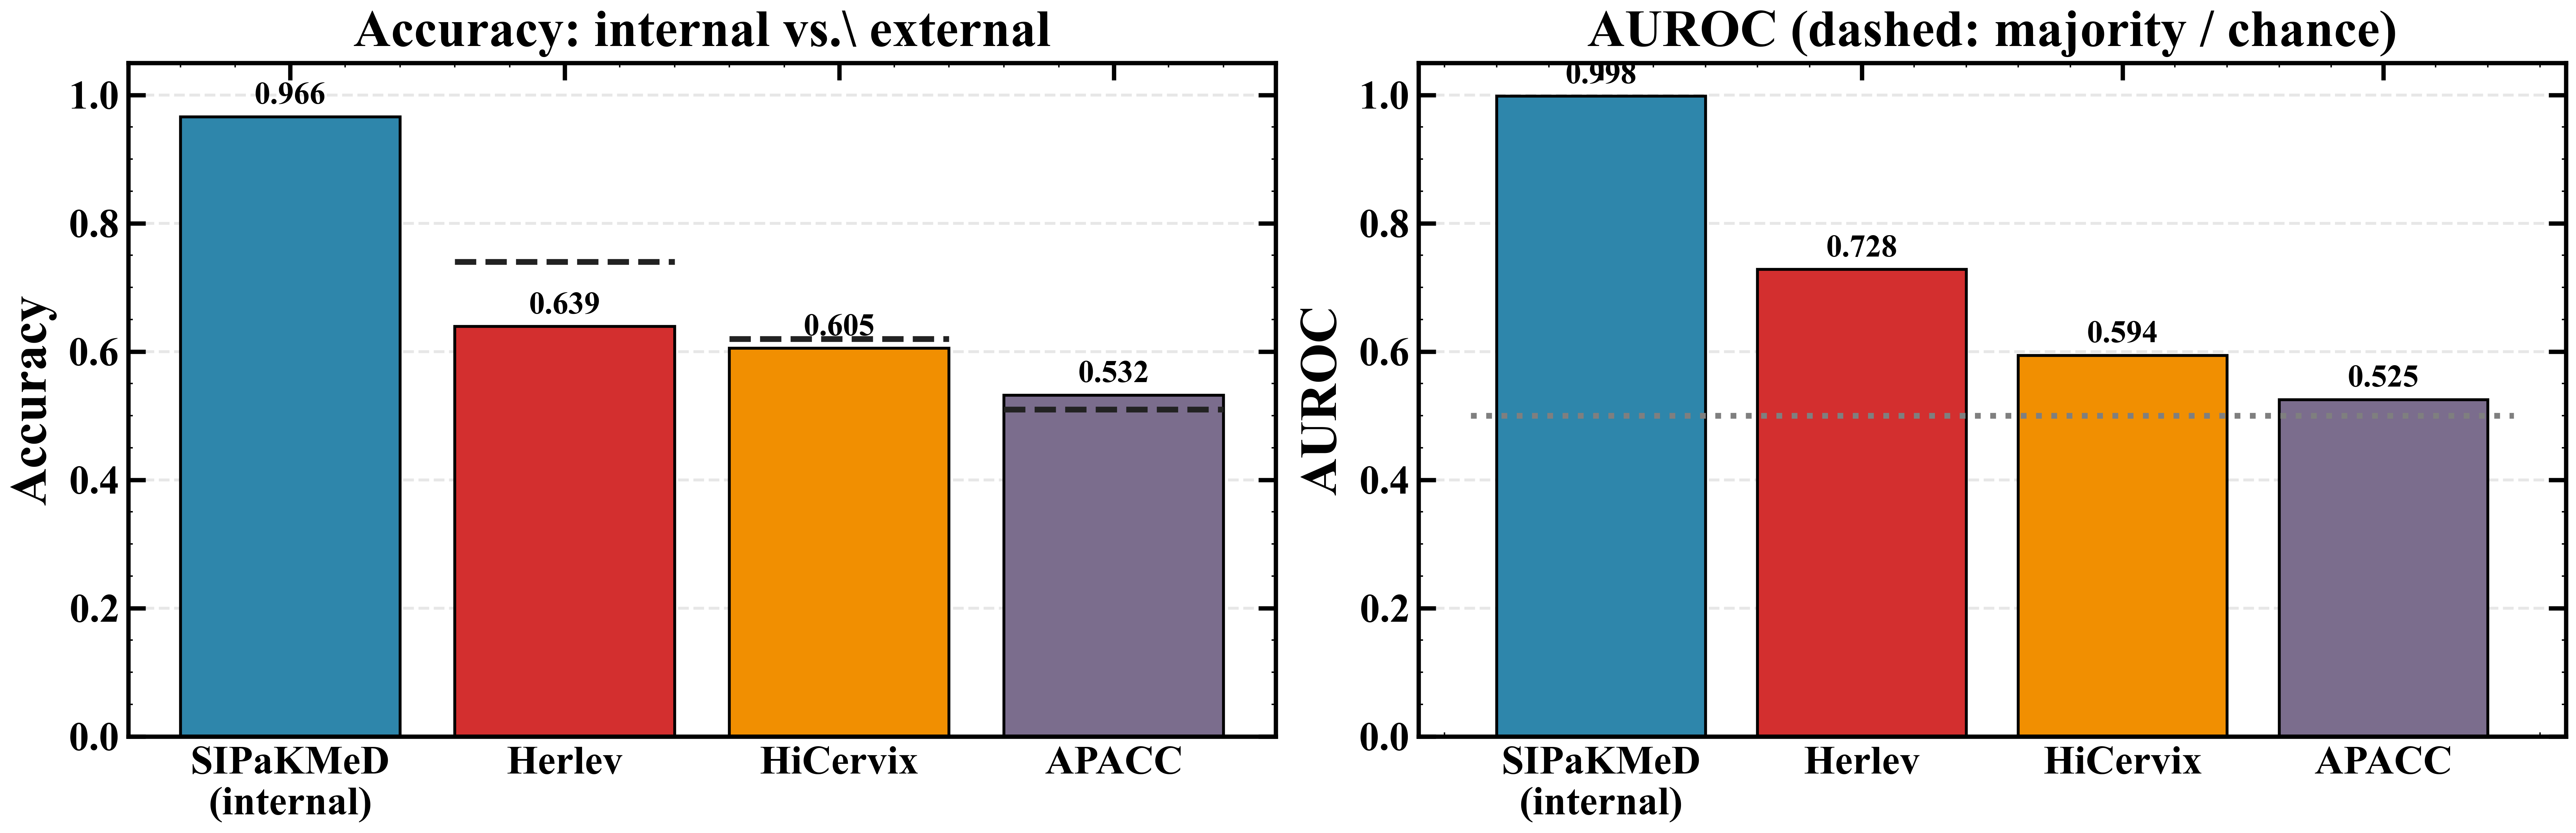
\includegraphics[width=0.92\textwidth]{teaser.png}
  \caption{\textbf{Internal excellence, external collapse.} The distilled student is excellent
  \emph{within} \sipakmed\ (accuracy $0.966$, AUROC $0.998$) but, evaluated unchanged on three
  external Papanicolaou datasets under a binary Normal/Abnormal alignment, collapses to
  $0.53\!-\!0.64$ accuracy and $0.53\!-\!0.73$ AUROC. Dashed lines mark the per-dataset majority-class
  baseline (left) and chance (right): at a fixed threshold the model falls \emph{below} the trivial
  baseline on two of three datasets despite retaining above-chance ranking signal. Severity tracks
  slide-preparation distance from \sipakmed's conventional smear.}
  \label{fig:teaser}
\end{figure*}

We subject a representative high-accuracy system to exactly such a measurement. We study a
knowledge-distilled classifier~\cite{hinton2015distilling} in which an EfficientNet-B4
teacher~\cite{tan2019efficientnet}, ImageNet-pretrained~\cite{deng2009imagenet} and trained on the
five \sipakmed\ cytomorphology classes, is distilled into a compact EfficientNet-B0 student. The
student is attractive for deployment---$4.67$\,M parameters against the teacher's $18.5$\,M---and we
ask whether such compression sacrifices accuracy, calibration, explainability, or generalisation. We
then evaluate the \emph{same} student, without retraining, across three independent Papanicolaou
datasets---\herlev~\cite{jantzen2005herlev}, \apacc, and \hicervix~\cite{cai2024hicervix}---that
differ in staining, segmentation and slide preparation (conventional smear, auto-segmented crops, and
liquid-based cytology). Because the five \sipakmed\ morphology classes do not share a label space
with the dysplasia and Bethesda~\cite{nayar2015bethesda} schemes of those datasets, we align them at
the only common, deterministically mappable level---a binary Normal-versus-Abnormal decision---with
glandular and out-of-scope categories explicitly excluded and the excluded fraction reported.

In-distribution the model is genuinely strong: the distilled student reaches accuracy $0.966$ and
\emph{exceeds its teacher on every metric}, is well calibrated (ECE\,$0.015$), and produces
cytologically plausible Grad-CAM~\cite{selvaraju2017gradcam} attributions. Out-of-distribution it
\emph{collapses} (\cref{fig:teaser}): binary accuracy falls to $0.639$ (\herlev), $0.605$ (\hicervix)
and $0.532$ (\apacc)---below the majority baseline on two of three sets---and AUROC to $0.73$, $0.59$,
$0.53$. The central scientific question is then \emph{why}, and in particular whether the failure is
a labelling/mapping artefact or a genuine model failure. We show it is the latter: the $\pabn$ score
ranks abnormal above normal cells in \emph{every} dataset (all AUROC$>0.5$), so the mapping is
correctly oriented; the collapse is genuine domain shift compounded by an operating-point
miscalibration that does not transfer across domains~\cite{guo2017calibration}, the cytology analogue
of shortcut learning~\cite{geirhos2020shortcut}. We make four contributions.

\begin{itemize}[leftmargin=1.2em,itemsep=1pt,topsep=2pt]
\item \textbf{C1 (a failure mode, characterised).} A reproducible cross-dataset audit showing that a
high-accuracy, well-calibrated, explainable distilled cytology model collapses on three independent
Pap datasets---below the majority baseline at a fixed threshold (\cref{sec:analysis}).
\item \textbf{C2 (a diagnosis, not just a number).} A methodology that mechanistically separates a
labelling artefact from genuine domain failure via class-conditional $\pabn$ separation, an
AUROC-above-chance test, and an accuracy-versus-majority-baseline / oracle-threshold analysis;
applied here it rules out relabelling and isolates domain shift $+$ operating-point miscalibration
(\cref{sec:analysis}).
\item \textbf{C3 (distillation paradox).} Evidence that distillation yields a \emph{smaller-yet-stronger}
in-distribution model---the B0 student surpasses its B4 teacher on every metric---which nonetheless
fails out-of-distribution, decoupling compression quality from generalisation (\cref{sec:exp}).
\item \textbf{C4 (honest evaluation).} We show the internal $0.966$ is itself optimistic
(same-field-of-view leakage), and give evidence-led remedies: leakage-safe cluster-grouped splits,
stain/domain normalisation~\cite{macenko2009stain}, per-domain calibration, and reporting
threshold-free AUROC with the excluded fraction (\cref{sec:discussion}).
\end{itemize}

\noindent\textbf{Paper organisation.} \Cref{sec:questions} states the research questions, hypotheses
and novelty; \cref{sec:primer} fixes cytology background and notation; \cref{sec:related} reviews
related work; \cref{sec:problem} defines the datasets and label alignment; \cref{sec:method} details
the data and training pipeline; \cref{sec:exp} reports in-distribution results; \cref{sec:analysis}
presents the cross-dataset collapse and its diagnosis; \cref{sec:discussion} discusses scope and
remedies.

\section{Research questions, hypotheses, and novelty}
\label{sec:questions}

A cervical-cytology classifier ships a single headline accuracy, but whether that number reflects
transferable diagnostic competence has not been examined systematically for distilled, edge-oriented
models. We ask whether the number can be trusted off its training distribution and, where it cannot,
\emph{why}. Stated precisely, the object of study is:

\begin{quote}
Given a model $f$ trained on the \sipakmed\ five-class space and reported at high in-distribution
accuracy, determine whether $f$ \textbf{(a)} retains discriminative skill on independent Pap datasets
under a deterministic binary alignment, \textbf{(b)} remains calibrated and explainable there, and
\textbf{(c)} if it fails, whether the failure is attributable to the label mapping or to a genuine
model/domain effect---using only frozen evaluation, documented mappings, and reported excluded
fractions.
\end{quote}

\subsection{Research questions and hypotheses}
\label{sec:rqs}

We organise the study around four research questions, each with the hypothesis we set out to test.

\begin{description}[leftmargin=1.4em,itemsep=3pt,topsep=3pt]
\item[RQ1 (compression vs.\ skill).] \emph{Can a knowledge-distilled B0 student match the B4 teacher's
in-distribution accuracy at a fraction of the parameters?}\\
\textbf{H1:} yes; the regularising effect of distillation may let the $4.67$\,M-parameter student
match or even exceed the $18.5$\,M teacher. (Answered in \cref{sec:exp}.)

\item[RQ2 (does accuracy transfer?).] \emph{Does strong in-distribution accuracy translate to
cross-dataset generalisation on independent Pap datasets?}\\
\textbf{H2:} no; a large internal-to-external gap is expected because the model sees a single
preparation protocol. (Answered in \cref{sec:analysis}.)

\item[RQ3 (artefact or genuine failure?).] \emph{Is any cross-dataset failure a label-mapping
artefact or a genuine model-and-domain failure?}\\
\textbf{H3:} genuine domain shift compounded by miscalibration, \emph{not} a labelling error---the
decision score should remain correctly oriented (abnormal ranked above normal) even as accuracy
falls. (Answered in \cref{sec:analysis}.)

\item[RQ4 (does trust transfer?).] \emph{Do calibration and explainability hold, and does calibration
transfer out-of-distribution?}\\
\textbf{H4:} in-distribution the model is well calibrated~\cite{guo2017calibration} and its Grad-CAM
attributions are cytologically plausible, but the calibrated operating point does \emph{not} transfer
across domains. (Answered in \cref{sec:exp,sec:analysis}.)
\end{description}

\subsection{What is novel}
\label{sec:novelty}

Our novelty is \emph{not} ``cross-dataset evaluation'' in general---generalisation testing is mature.
It is the specific, rarely-occupied intersection of three things in the cervical-cytology setting.

\begin{enumerate}[leftmargin=1.5em,itemsep=2pt,topsep=2pt]
\item \textbf{A deterministic, leakage-aware, multi-dataset audit} of a distilled cytology model
across three external Pap datasets (\herlev, \apacc, \hicervix) under a documented binary crosswalk
with \emph{reported excluded fractions}---rather than a single-dataset accuracy or an undocumented
relabelling that silently inflates the score.
\item \textbf{A mechanistic diagnosis that distinguishes a label artefact from domain failure.} We
introduce a simple, decisive test---the class-conditional $\pabn$ separation together with the
AUROC$>0.5$ criterion---and an accuracy-versus-majority-baseline / oracle-threshold analysis that
localises the failure to operating-point miscalibration and slide-preparation distance. This turns
``it does not generalise'' into ``here is the cause.''
\item \textbf{The distillation paradox made explicit.} We show the compressed student is
\emph{stronger} than its teacher in-distribution yet fails identically out-of-distribution, evidence
that compression quality and generalisation are decoupled and that distillation does not confer
robustness~\cite{geirhos2020shortcut}.
\end{enumerate}

\noindent\textbf{Contrast with the closest practice.} The standard report is a single in-distribution
accuracy; we show it is optimistic (leaky split) and non-transferable. Where external sets are used,
the label crosswalk is frequently undocumented; we make it deterministic and report what is excluded.
And where a drop is observed, it is typically attributed loosely to ``domain shift''; we provide a
test that \emph{rules out} the competing artefact explanation and pinpoints the operative mechanism.

\subsection{Outcome of the hypotheses}
\label{sec:hyp-status}

Each hypothesis's outcome is summarised in \cref{tab:hyp-status}. Reporting that the headline accuracy
fails to transfer---and that the internal estimate is itself optimistic---is the deliberate point: an
audit is worthless if it suppresses its own inconvenient findings.

\begin{table*}[tb]
\centering\small
\caption{\textbf{Where each hypothesis stands.} All four are supported; the load-bearing result is
H3---the cross-dataset collapse is a \emph{genuine} domain/calibration failure, not an artefact of
the binary label alignment.}
\label{tab:hyp-status}
\begin{tabular}{@{}l p{0.40\textwidth} p{0.33\textwidth} l@{}}
\toprule
Hyp. & Claim (abbreviated) & Verdict & Where \\
\midrule
H1 & distilled B0 matches/exceeds the B4 teacher in-distribution & \textbf{Supported} (student $>$ teacher on all metrics) & \cref{sec:exp} \\
H2 & strong in-distribution accuracy does not transfer cross-dataset & \textbf{Supported} ($33$--$43$-pt drop) & \cref{sec:analysis} \\
H3 & failure is domain shift $+$ miscalibration, not a label artefact & \textbf{Supported} ($\pabn$ separation $>0$, AUROC$>0.5$) & \cref{sec:analysis} \\
H4 & in-distribution calibration holds but does not transfer & \textbf{Supported} (binary ECE $0.008$ in; $0.22$--$0.33$ out) & \cref{sec:exp,sec:analysis} \\
\bottomrule
\end{tabular}
\end{table*}

\section{Background and notation}
\label{sec:primer}

\noindent\textbf{Cervical cytology.} A Papanicolaou (Pap) test stains exfoliated cervical cells;
a cytologist reads the slide for morphological signs of (pre)malignancy. Two labelling traditions
coexist. \emph{Morphology} schemes name the cell type or change---\sipakmed\ uses five classes:
Superficial-Intermediate, Parabasal, Metaplastic (normal/benign squamous), and Koilocytotic,
Dyskeratotic (abnormal squamous changes)~\cite{plissiti2018sipakmed}. \emph{Diagnostic} schemes name
the lesion grade---the WHO dysplasia scale (\herlev) and the Bethesda system (NILM, ASC-US, LSIL,
ASC-H, HSIL, SCC; plus glandular AGC)~\cite{nayar2015bethesda}. These taxonomies are not in
correspondence: a Bethesda grade does not determine a morphology class and vice versa, which is the
crux of the cross-dataset label problem (\cref{sec:problem}).

\noindent\textbf{Slide preparation.} Slide preparation is a first-order source of appearance shift
even when the stain is Pap. Conventional smears (\sipakmed, \herlev) differ from liquid-based cytology
(\hicervix), which differs again from auto-segmented single-cell crops (\apacc); each changes cell
density, background, focus and segmentation. We will see the cross-dataset collapse is ordered by this
preparation distance.

\noindent\textbf{Notation.} A model $f$ maps a cell image $x$ to class logits $z\in\mathbb{R}^5$ over
the \sipakmed\ classes; $\softmax(z)$ are the class probabilities and $\hat{y}=\arg\max_k z_k$ the
prediction. For binary cross-dataset scoring we collapse to a single abnormality score
\begin{equation}
\pabn \;=\; \softmax(z)_{\mathrm{Koilo}} + \softmax(z)_{\mathrm{Dysk}},
\label{eq:pabn}
\end{equation}
i.e.\ the probability mass on the two abnormal morphology classes, thresholded at $\tau$ (default
$0.5$). Calibration is measured by the expected calibration error (ECE), the gap between confidence
and accuracy averaged over confidence bins~\cite{guo2017calibration}.

\section{Related work}
\label{sec:related}

\noindent\textbf{Deep learning for cervical cytology.} Curated single-cell benchmarks---\sipakmed's
five Pap morphology classes~\cite{plissiti2018sipakmed} and the older \herlev\ WHO-dysplasia
set~\cite{jantzen2005herlev}---have driven a large body of work reporting near-ceiling within-dataset
accuracy with convolutional backbones, and recent liquid-based resources such as
\hicervix~\cite{cai2024hicervix} extend this with hierarchical Bethesda labels. The near-universal
protocol, however, trains and tests on one collection, leaving transfer to other slide-preparation
pipelines unmeasured.

\noindent\textbf{Knowledge distillation for efficient medical models.}
Distillation~\cite{hinton2015distilling} compresses a high-capacity teacher into a deployable student
and is widely used for edge-oriented medical imaging. Reported gains are almost always
in-distribution; whether a distilled student inherits the teacher's (lack of) robustness is rarely
tested. We find the student can be \emph{stronger} than its teacher in-distribution yet equally
fragile out-of-distribution.

\noindent\textbf{Generalisation and shortcut learning.} Deep classifiers frequently latch onto
dataset-specific cues---stain, scanner, segmentation, background---rather than the causal
signal~\cite{geirhos2020shortcut}; in histopathology and cytology this manifests as sharp accuracy
drops across sites. Our diagnosis localises the cytology version of this effect to slide-preparation
distance and a non-transferable operating point.

\noindent\textbf{Calibration and explainability in medical imaging.} Modern networks are
miscalibrated~\cite{guo2017calibration}; calibration is especially load-bearing for screening, where a
decision threshold must be trusted. Grad-CAM~\cite{selvaraju2017gradcam} is the standard
attribution tool. We report both, and show in-distribution calibration that does \emph{not} survive
domain shift---a failure mode that a single ECE number, measured in-distribution, hides.

\noindent\textbf{Cross-dataset label alignment.} Morphology and Bethesda taxonomies do not map
one-to-one, and stain-normalisation~\cite{macenko2009stain} only addresses appearance, not labels.
Prior cross-dataset cytology comparisons often relabel informally; we instead fix a deterministic
many-to-one binary crosswalk and report the excluded fraction as an honesty metric.

\section{Problem setup: data and label alignment}
\label{sec:problem}

\noindent\textbf{Datasets.} We train on \sipakmed---$5{,}015$ Pap images
($4{,}049$ cropped single cells $+$ $966$ cluster field-of-view images) in five morphology classes,
conventional smear---and evaluate, frozen, on three external single-cell Pap sets
(\cref{tab:datasets}): \herlev\ ($917$
cells, $7$ WHO-dysplasia classes, conventional smear), \apacc\ ($1{,}125$ auto-segmented crops, coarse
healthy/unhealthy), and \hicervix\ ($4{,}823$ scorable of $8{,}051$ test cells, hierarchical Bethesda,
liquid-based). The three external sets deliberately span the preparation axis of \cref{sec:primer}.

\begin{table*}[tb]
\caption{\textbf{Datasets.} \sipakmed\ is the sole training source; the others are frozen external
evaluation sets spanning slide preparations and incompatible native label spaces.}
\label{tab:datasets}
\centering\small
\begin{tabular}{@{}lllll@{}}
\toprule
Dataset & Role & Preparation / type & Native labels & Size \\
\midrule
\sipakmed~\cite{plissiti2018sipakmed} & Train ($+$val) & Conventional smear; cells $+$ FoV & 5 cytomorphology & $5{,}015$ imgs ($4{,}049$ cells) \\
\herlev~\cite{jantzen2005herlev}      & External eval & Conventional smear; single cells & 7 WHO dysplasia & $917$ cells \\
\apacc                                 & External eval & Auto-segmented single-cell crops & 4 coarse & $1{,}125$ cells \\
\hicervix~\cite{cai2024hicervix}       & External eval & Liquid-based cytology (LBC) & Hierarchical Bethesda & $4{,}823$ ($8{,}051$ total) \\
\bottomrule
\end{tabular}
\end{table*}

\noindent\textbf{Why a binary alignment.} The five \sipakmed\ morphology classes do not share a label
space with the WHO/Bethesda grades of the external sets: projecting a grade onto a morphology class is
one-to-many or undefined (e.g.\ NILM may be any of three normal morphologies; LSIL spans Koilocytotic
and Dyskeratotic). The only level at which \emph{both} the model's prediction and the native label map
\emph{deterministically and many-to-one} is the binary Normal-versus-Abnormal decision. We therefore
score the abnormality mass $\pabn$ (\cref{eq:pabn}) at threshold $\tau{=}0.5$ against a binary
ground truth obtained from the crosswalk in \cref{tab:mapping}.

\noindent\textbf{The crosswalk and its honesty gate.} \cref{tab:mapping} lists the deterministic map.
On the model side, $\{$Superficial-Intermediate, Parabasal, Metaplastic$\}\!\to\!$Normal and
$\{$Koilocytotic, Dyskeratotic$\}\!\to\!$Abnormal. On the label side, normal squamous and benign
categories map to Normal and dysplastic/SIL categories to Abnormal. Crucially, \emph{glandular and
out-of-scope native classes have no squamous home in the five-class space and are excluded}: \herlev\
\emph{columnar}, \hicervix\ \emph{AGC} (glandular) and \emph{microbe}, and \apacc\ \emph{rubbish}/
\emph{bothcells}. We report the excluded fraction per dataset, because silently dropping hard,
unmappable cells would inflate the binary score. This deterministic, documented mapping is what lets
us later attribute the cross-dataset collapse to the model rather than to the labels.

\begin{table*}[tb]
\caption{\textbf{Binary label crosswalk.} Deterministic Normal/Abnormal mapping; the model-side
decision is $\pabn$ (\cref{eq:pabn}). Glandular and out-of-scope native categories are excluded and
their fraction reported.}
\label{tab:mapping}
\centering\small
\begin{tabular}{@{}lll@{}}
\toprule
Source & $\rightarrow$ Normal & $\rightarrow$ Abnormal \quad(/ Excluded) \\
\midrule
\sipakmed\ (model) & Superficial-Interm., Parabasal, Metaplastic & Koilocytotic, Dyskeratotic \\
\herlev & superficiel, intermediate, columnar$^\dagger$ & light/moderate/severe dyspl., carcinoma-in-situ \\
\apacc & healthy & unhealthy \quad(rubbish, bothcells excl.) \\
\hicervix & \texttt{level\_1}{=}negative & \texttt{level\_1}{=}ASC \quad(AGC, microbe excl.) \\
\bottomrule
\end{tabular}\\[2pt]
{\footnotesize $^\dagger$\herlev\ columnar (glandular) is mapped to Normal in this legacy crosswalk; a
stricter variant excludes it. The choice moves the headline by $<\!1$ point and does not affect the
diagnosis (\cref{sec:analysis}).}
\end{table*}

\section{Data and training pipeline}
\label{sec:method}

\subsection{Exploratory data analysis}
\label{sec:eda}
Before training we characterise \sipakmed\ (\cref{fig:eda}). Three facts shape the pipeline. (i)
\textbf{Mild class imbalance:} per-class totals range $895$ (Parabasal) to $1{,}064$ (Metaplastic),
an imbalance ratio of $1.19$---small enough to address with weighted loss rather than resampling.
(ii) \textbf{Strong size heterogeneity:} cell crops span $62\!-\!2048$\,px in width (mean $615$) and
$62\!-\!1536$\,px in height, mandating a fixed-size resize. (iii) \textbf{Dual granularity:} the corpus
mixes $966$ cluster field-of-view images with $4{,}049$ cropped single cells; we use both, as in the
original pipeline.

\begin{figure*}[tb]
  \centering
  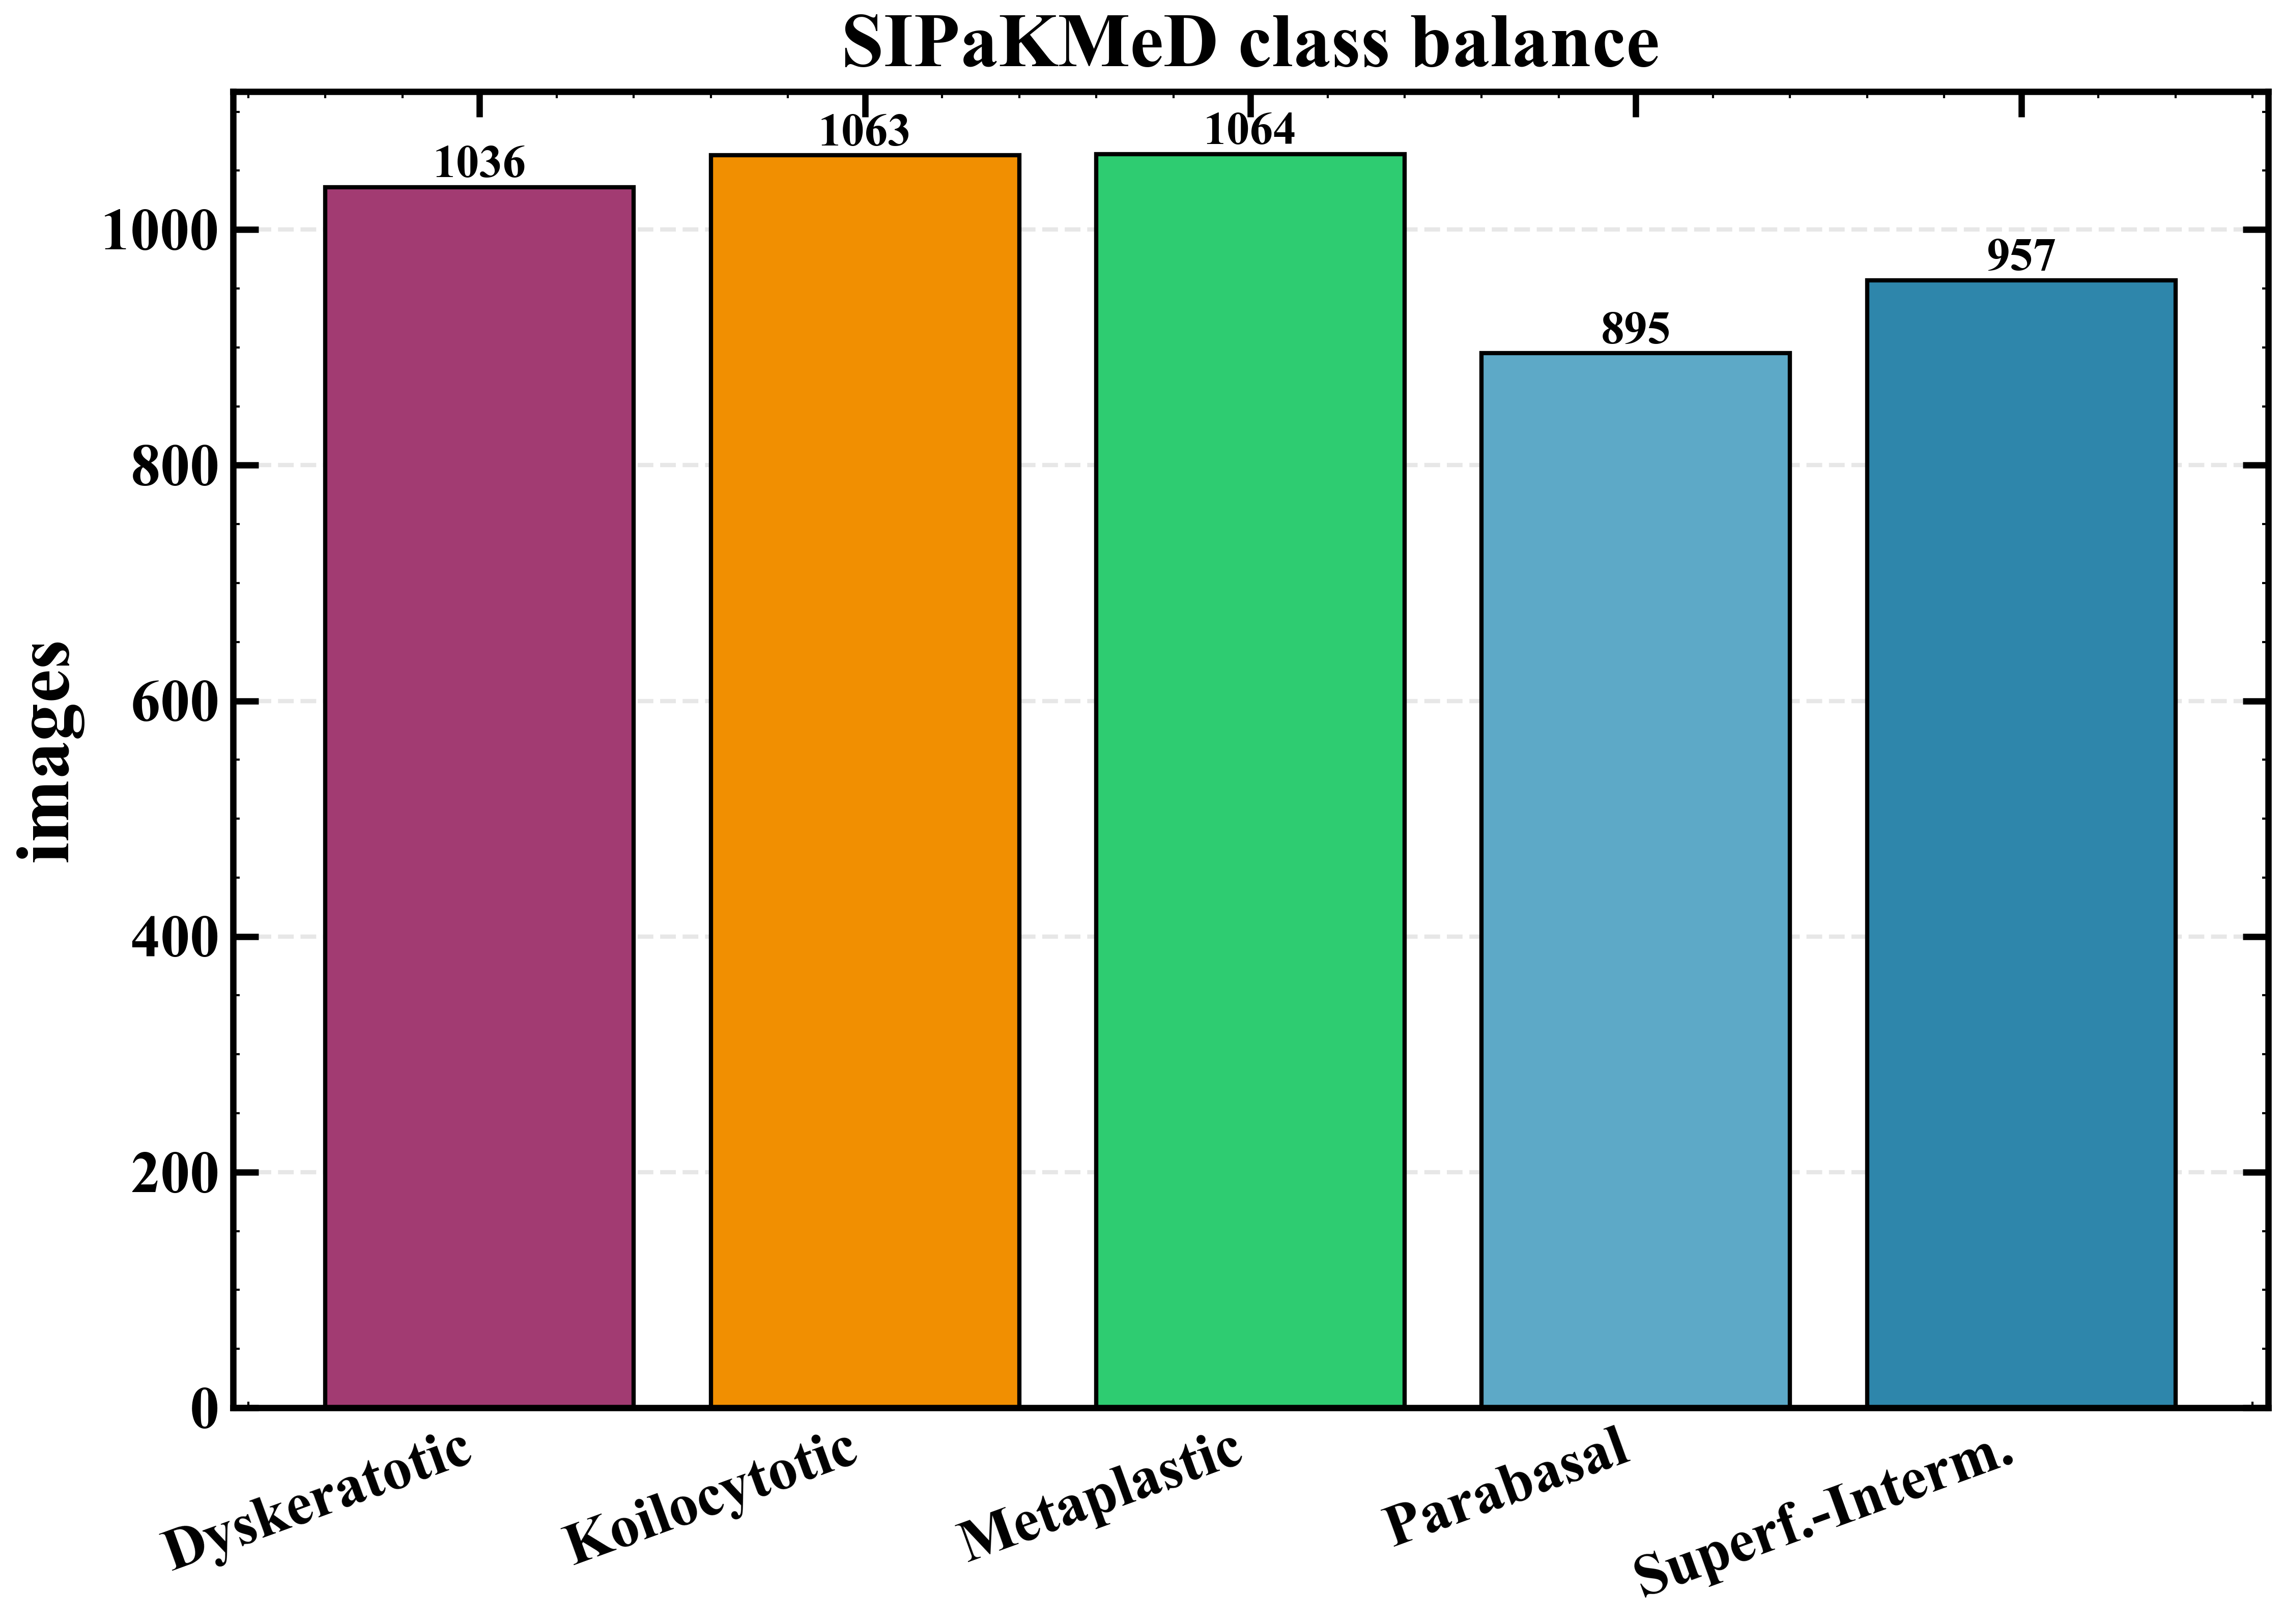
\includegraphics[width=0.40\textwidth]{eda_class_balance.png}\hfill
  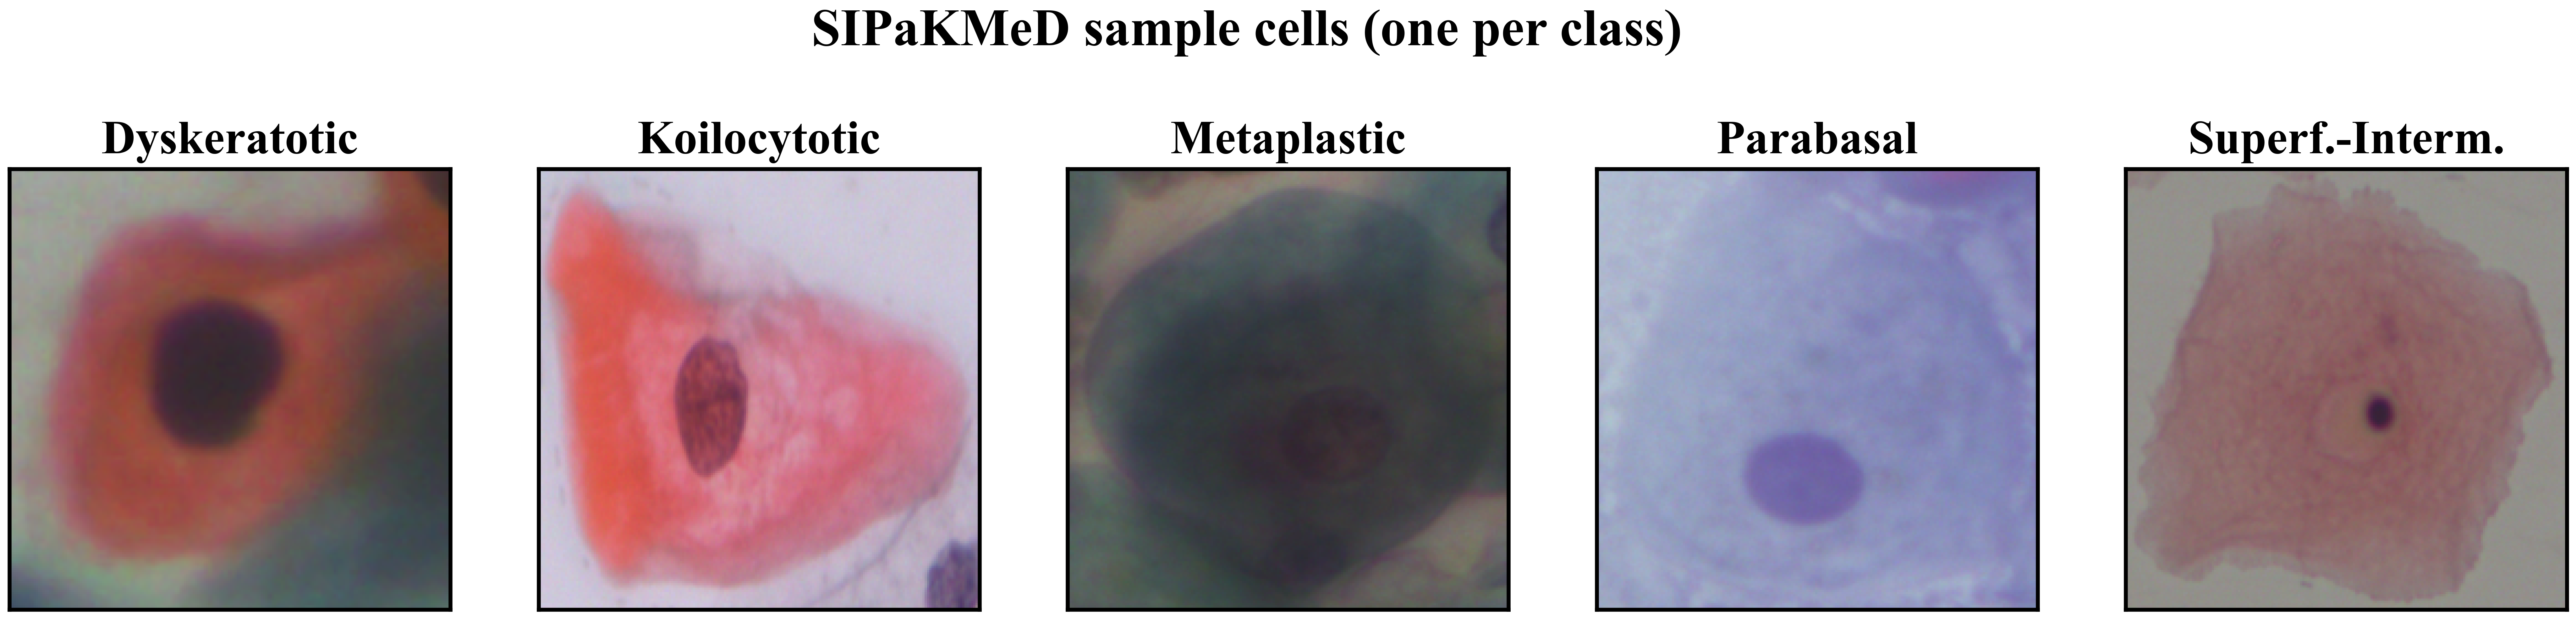
\includegraphics[width=0.56\textwidth]{eda_sample_cells.png}
  \caption{\textbf{Exploratory data analysis of \sipakmed.} Left: per-class image counts (mild
  imbalance, ratio $1.19$). Right: representative cells across the five morphology classes.}
  \label{fig:eda}
\end{figure*}

\subsection{Preprocessing and augmentation}
\label{sec:preproc}
Images are decoded to RGB, resized to $380\!\times\!380$ (the B4 native resolution, used for both
teacher and student), and channel-normalised with ImageNet statistics~\cite{deng2009imagenet}.
Train-time augmentation is cytology-appropriate---cells have \emph{no canonical orientation}, so we
apply random horizontal and vertical flips ($p{=}0.5$ each), random rotation ($\pm72^{\circ}$), and
mild random affine scaling ($0.9\!-\!1.1$). We deliberately avoid heavy shear, elastic warps or strong
hue shifts, which distort nuclear morphology---the very signal that separates the classes. Evaluation
(in- and cross-distribution) uses resize and normalisation only, with no augmentation.

\subsection{Architecture}
\label{sec:arch}
Both models are EfficientNets~\cite{tan2019efficientnet} with ImageNet-pretrained backbones: a B4
teacher ($18.5$\,M parameters) and a B0 student ($4.67$\,M). The native classifier is replaced by a
head $\mathrm{BN}\!\to\!\mathrm{Linear}(\,\cdot\,,512)\!\to\!\mathrm{ReLU}\!\to\!\mathrm{Dropout}
\!\to\!\mathrm{Linear}(512,5)$.

\subsection{Two-stage teacher and knowledge distillation}
\label{sec:train}
The teacher is trained in two stages with Adam and class-weighted cross-entropy (weight
$\propto 1/\text{count}$), monitoring validation loss: \emph{stage 1} freezes the backbone (lr
$10^{-3}$, $\le 30$ epochs, ReduceLROnPlateau), \emph{stage 2} fine-tunes the whole network (lr
$10^{-5}$, $\le 50$ epochs). The student is then distilled with the Hinton
objective~\cite{hinton2015distilling}:
\begin{equation}
\begin{split}
\mathcal{L} = {}&\alpha\,\mathrm{CE}(y,z_s) \\
&+ (1-\alpha)\,T^2\,
\mathrm{KL}\!\big(\softmax(z_t/T)\,\|\,\softmax(z_s/T)\big),
\end{split}
\label{eq:kd}
\end{equation}
with temperature $T{=}4$ and $\alpha{=}0.1$ (so the soft teacher signal dominates), Adam (lr
$5\!\times\!10^{-5}$, $\le 40$ epochs), monitoring validation accuracy. Training uses BF16 mixed
precision on a single $16$\,GB consumer GPU, batch size $32$, seed $42$, and a per-class stratified
$80/20$ train/validation split ($4{,}012$ train, $1{,}003$ validation). The teacher converges in
$71$ epochs ($30$ frozen $+$ $41$ fine-tuning, early-stopped) and the student in $34$ epochs; both
validation curves track training, indicating no overfitting (\cref{sec:exp}). We flag here---and
quantify in \cref{sec:analysis}---that this random per-cell split leaks same-field-of-view cells
across train and validation, making the internal estimate optimistic.

\section{In-distribution results}
\label{sec:exp}

\subsection{Training dynamics}
Validation tracks training closely for both models (\cref{fig:curves}); there is no overfitting gap,
and early stopping halts the teacher at $71$ and the student at $34$ epochs. The distilled student's
validation accuracy converges above the teacher's, foreshadowing the result below.

\begin{figure*}[tb]
  \centering
  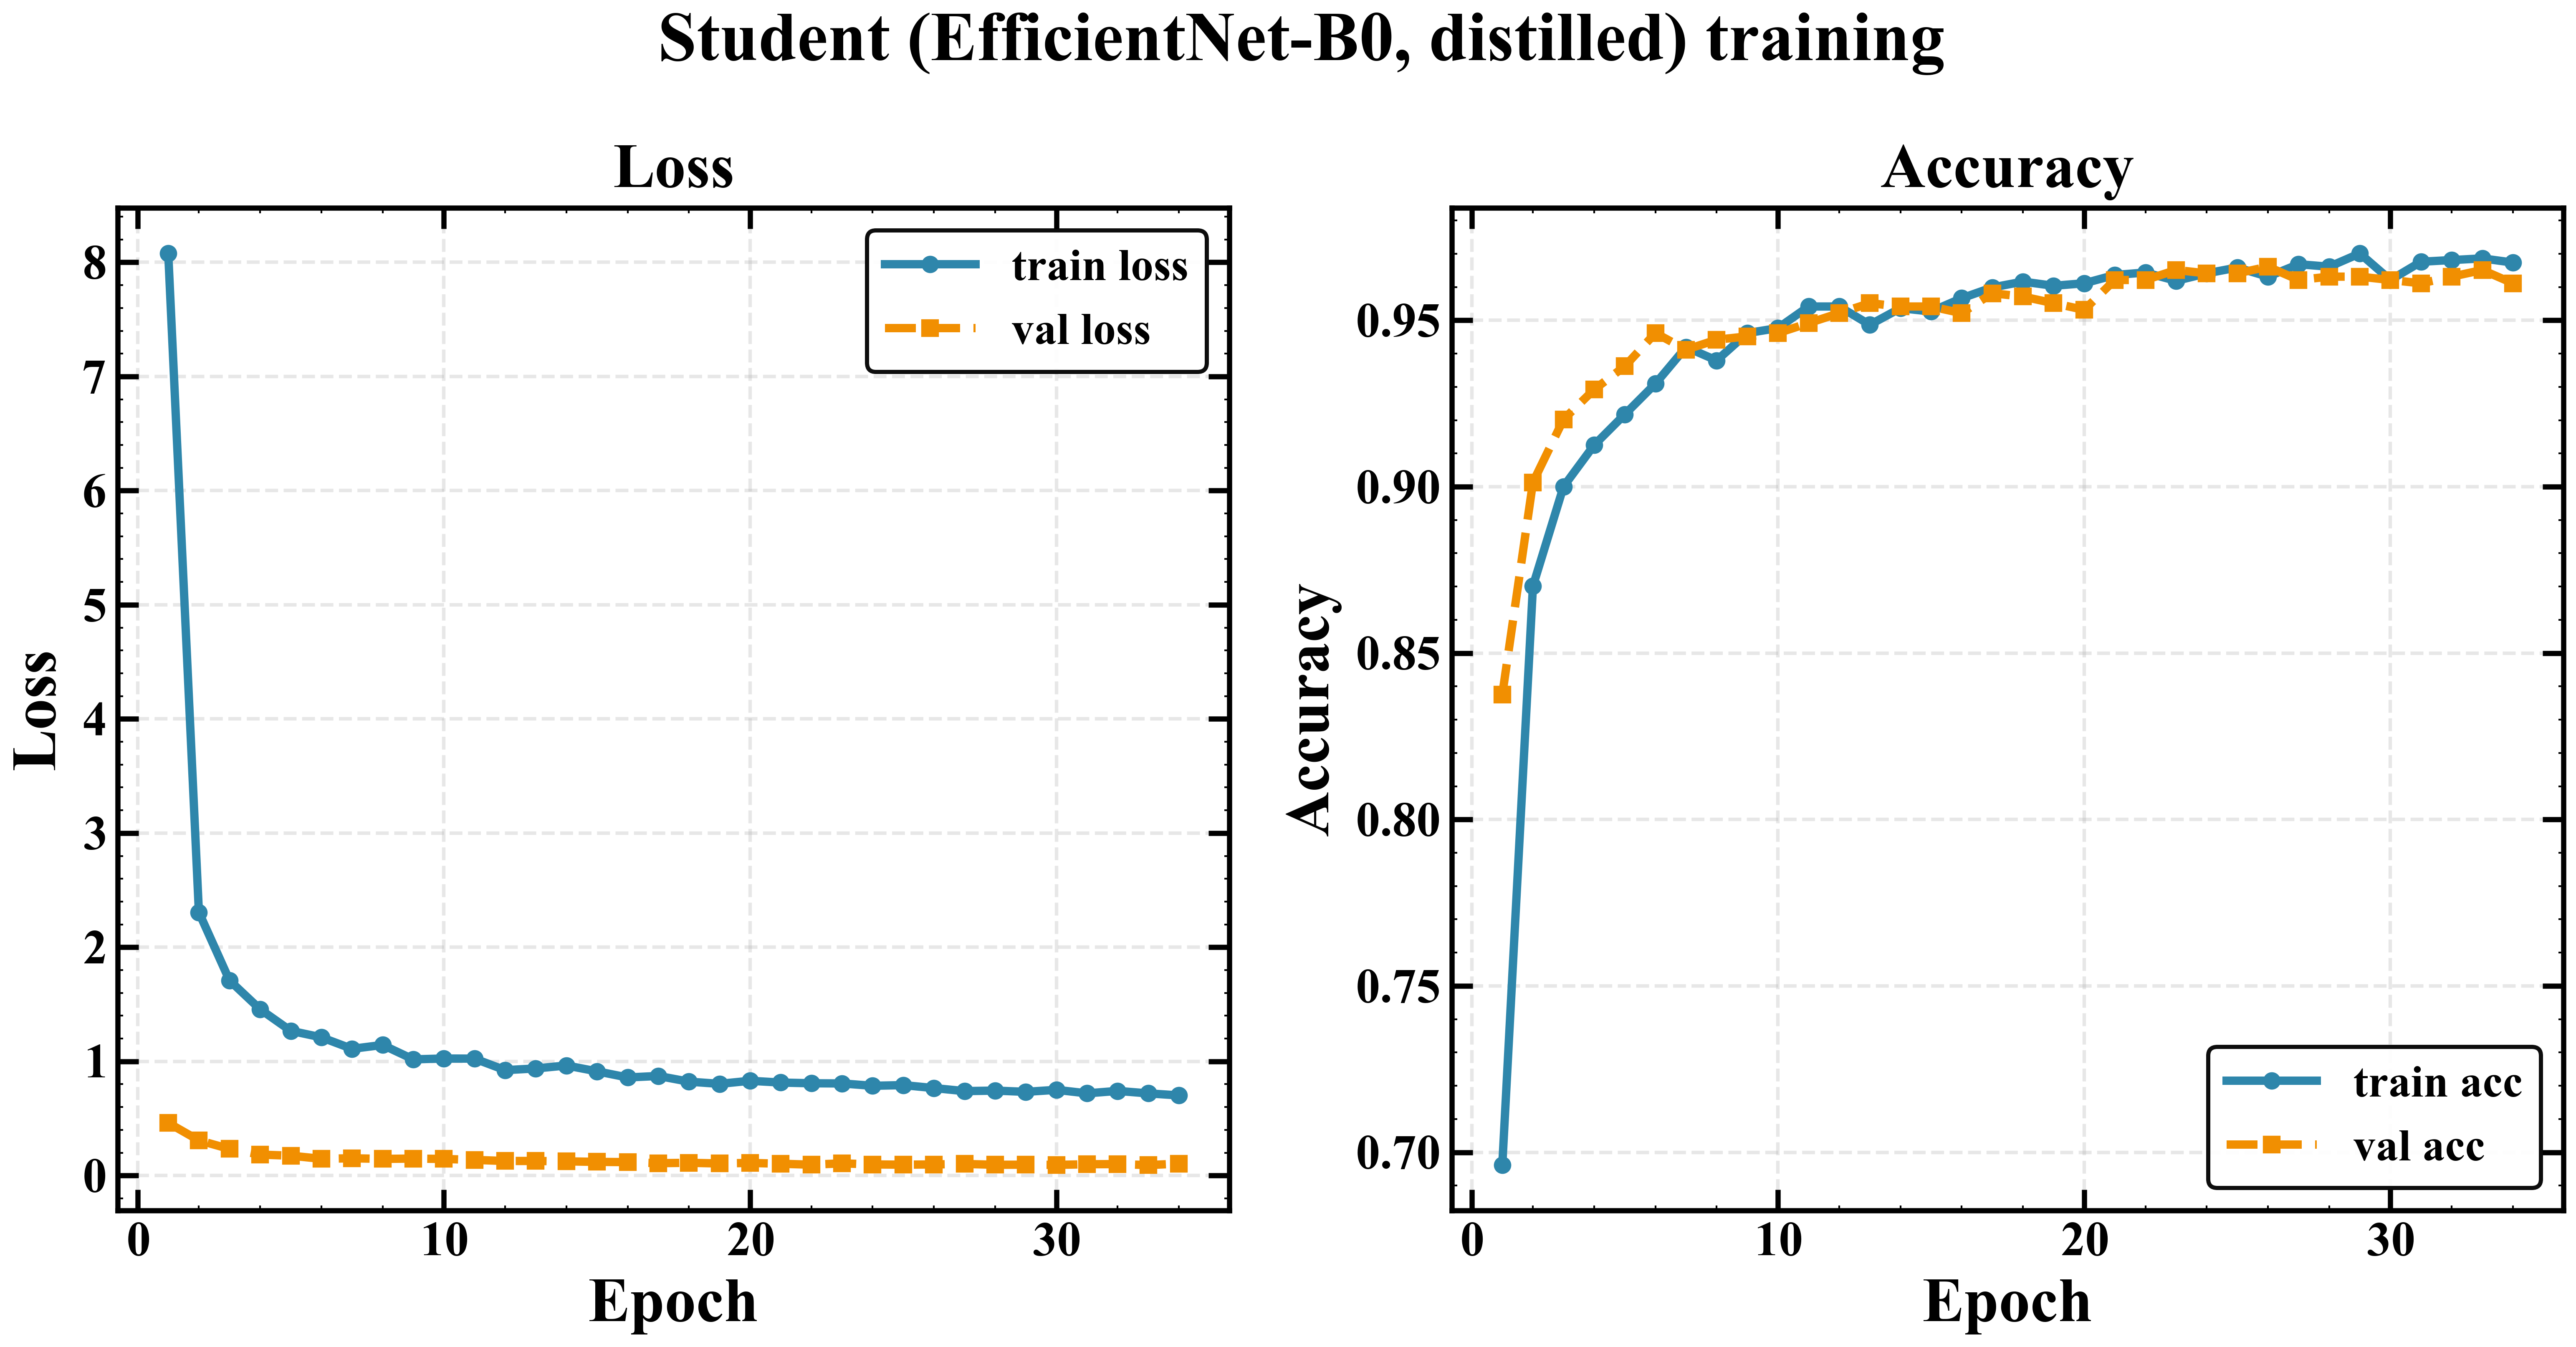
\includegraphics[width=0.49\textwidth]{student_training_curves.png}\hfill
  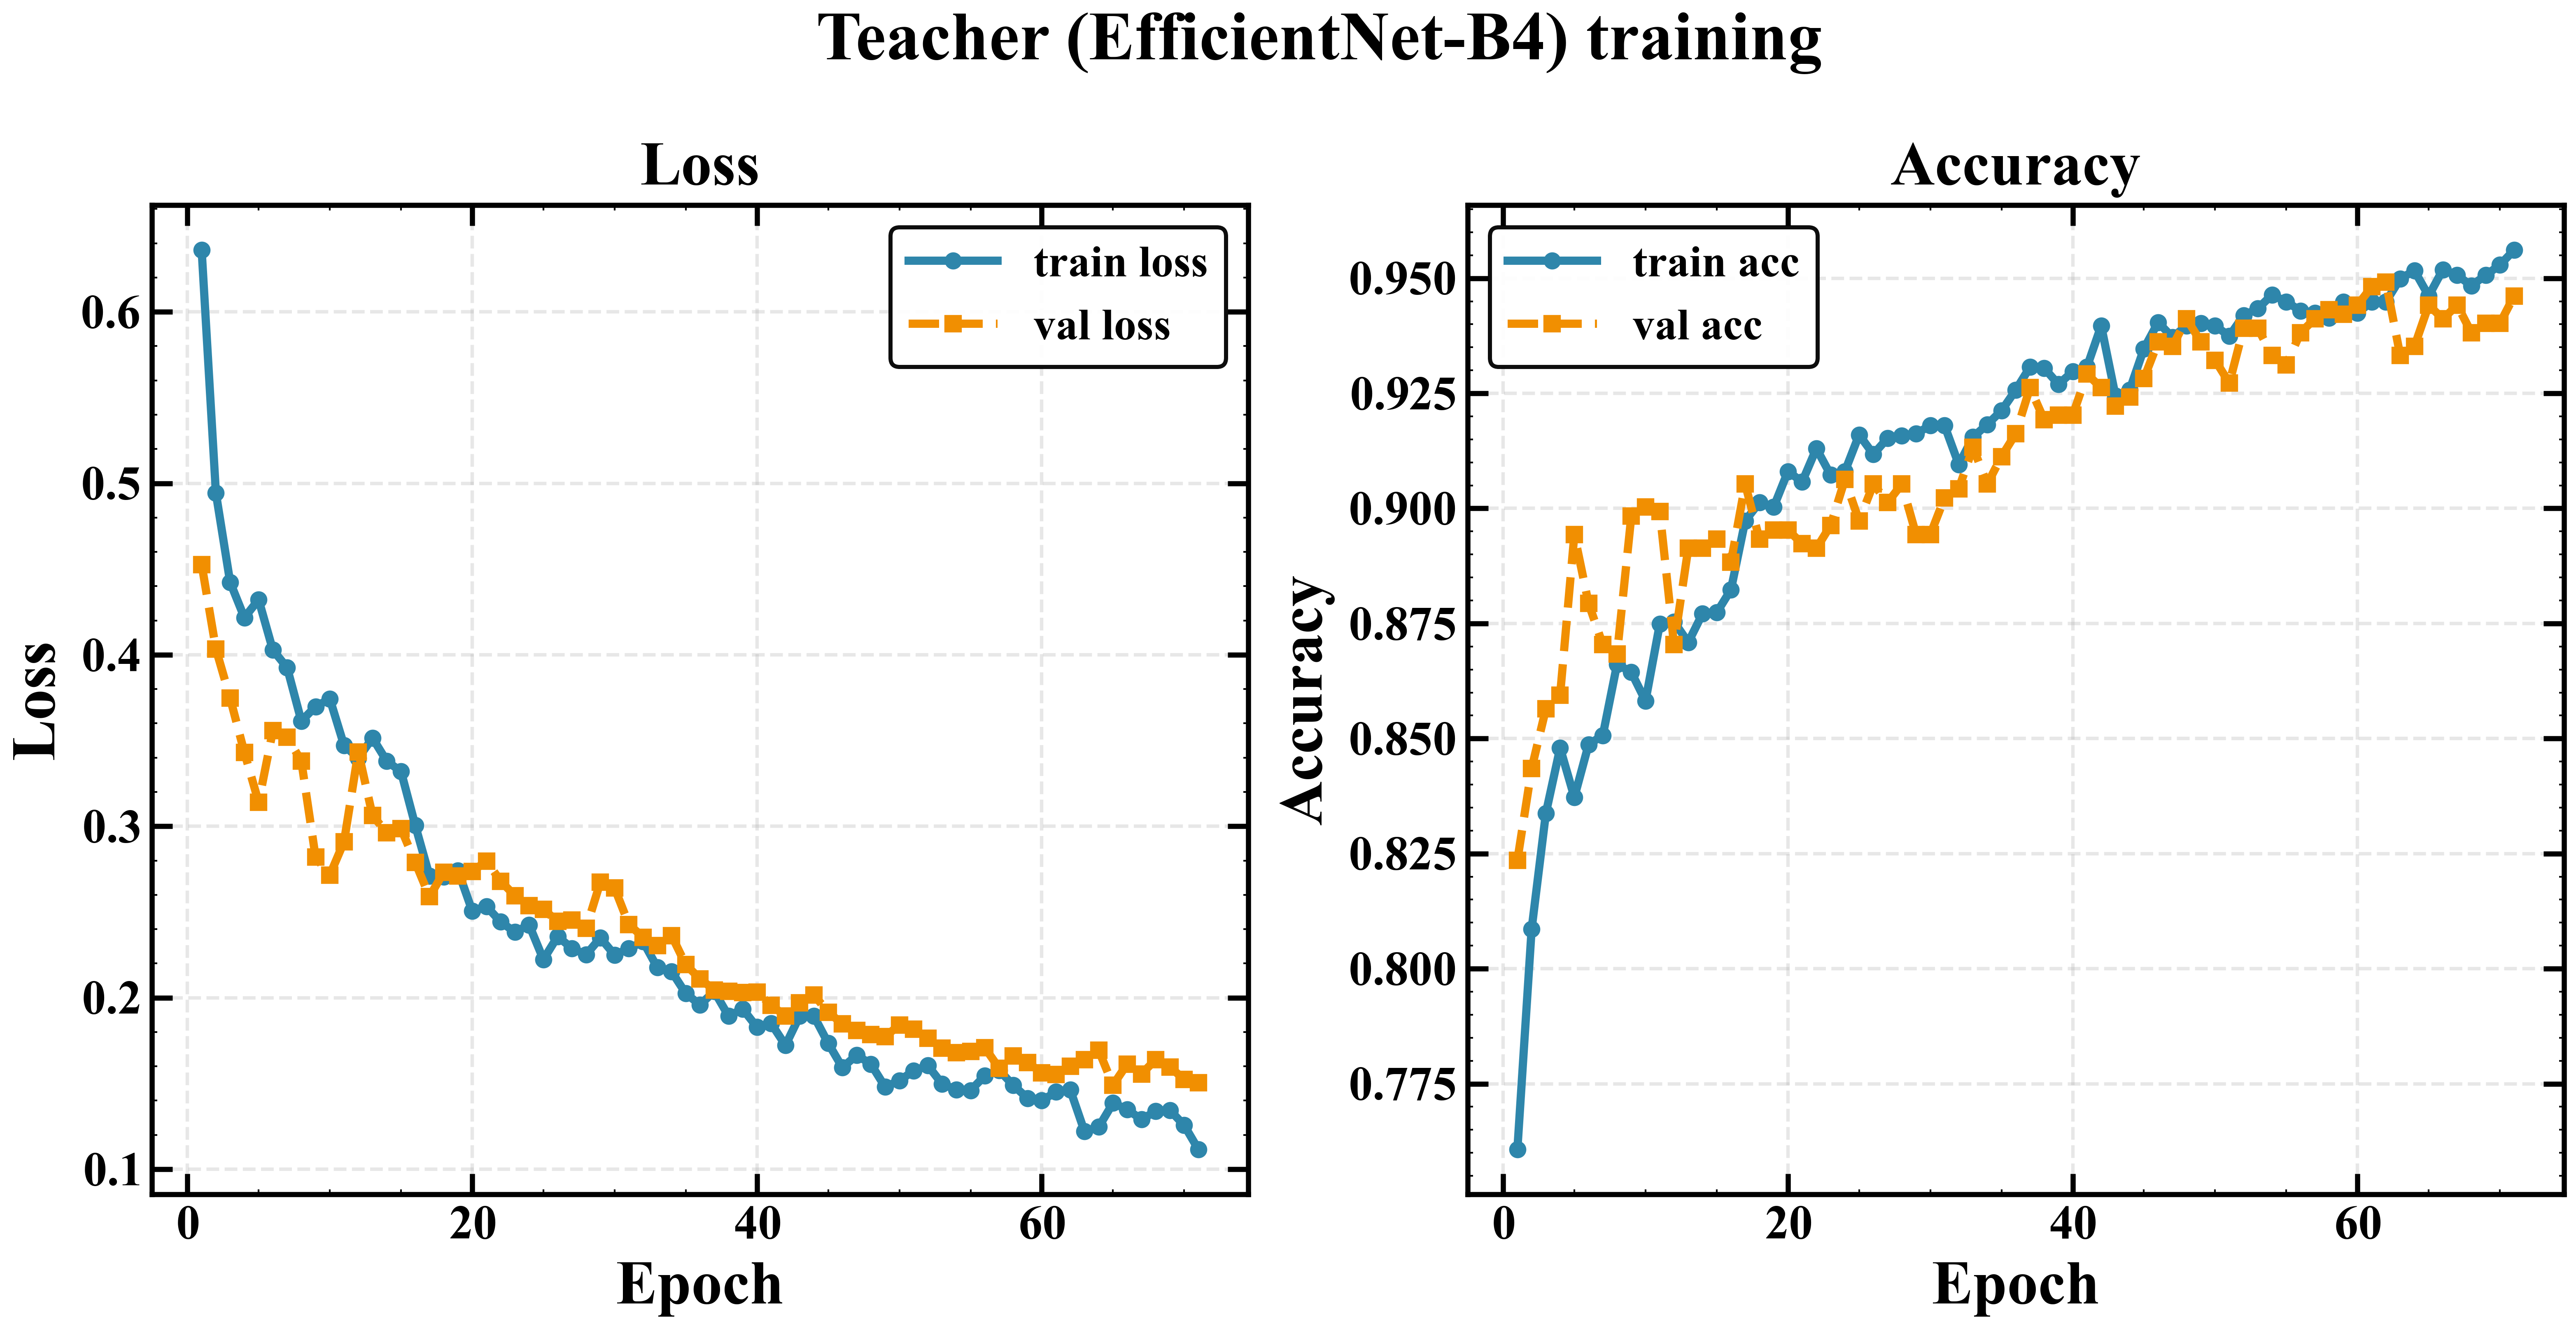
\includegraphics[width=0.49\textwidth]{teacher_training_curves.png}
  \caption{\textbf{Training dynamics.} Left: distilled B0 student ($34$ epochs). Right: B4 teacher
  (two stages, $71$ epochs). Validation tracks training in both---no overfitting.}
  \label{fig:curves}
\end{figure*}

\subsection{Classification performance (answering RQ1)}

\begin{table}[t]
\caption{\textbf{In-distribution five-class metrics.} \sipakmed\ validation, $n{=}1003$. The distilled
student surpasses its teacher on every metric and is well calibrated.}
\label{tab:indist}
\centering\small
\begin{tabular}{@{}lcc@{}}
\toprule
Metric & Teacher (B4) & \best{Student (B0)} \\
\midrule
Parameters         & 18.5\,M & \best{4.67\,M} \\
Accuracy           & 0.943 & \best{0.966} \\
Balanced accuracy  & 0.946 & \best{0.968} \\
Macro-$F_1$        & 0.945 & \best{0.967} \\
Cohen's $\kappa$   & 0.929 & \best{0.958} \\
AUROC (OvR macro)  & 0.995 & \best{0.998} \\
ECE (5-class)      & 0.013 & 0.015 \\
\bottomrule
\end{tabular}
\end{table}

\cref{tab:indist} reports the five-class metrics on the held-out \sipakmed\ validation split
($n{=}1003$). The distilled student reaches accuracy $0.966$, macro-$F_1$ $0.967$, Cohen's $\kappa$
$0.958$ and AUROC $0.998$, and \emph{exceeds the teacher on every metric} despite carrying $4\times$
fewer parameters---supporting \textbf{H1} and exposing a distillation paradox we return to in
\cref{sec:discussion}. The soft teacher targets evidently regularise the student rather than merely
compress it. Per-class (\cref{tab:perclass}, \cref{fig:cm}), the model is near-perfect on
Superficial-Intermediate and Parabasal ($F_1\,0.995/0.994$) and weakest on \emph{Koilocytotic}
($F_1\,0.919$, recall $0.873$), whose koilocytic halo overlaps morphologically with neighbouring
classes; this single class accounts for most of the in-distribution error.

\begin{table}[t]
\caption{\textbf{Per-class metrics (student).} Precision, recall and $F_1$ on the \sipakmed\
validation split. Koilocytotic is the weakest class.}
\label{tab:perclass}
\centering\small
\begin{tabular}{@{}lcccc@{}}
\toprule
Class & P & R & $F_1$ & $n$ \\
\midrule
Superficial-Intermediate & 0.990 & 1.000 & 0.995 & 191 \\
Parabasal                & 0.989 & 1.000 & 0.994 & 179 \\
Dyskeratotic             & 0.958 & 0.986 & 0.971 & 207 \\
Metaplastic              & 0.933 & 0.981 & 0.957 & 213 \\
Koilocytotic             & 0.969 & 0.873 & 0.919 & 213 \\
\bottomrule
\end{tabular}
\end{table}

\begin{figure}[t]
  \centering
  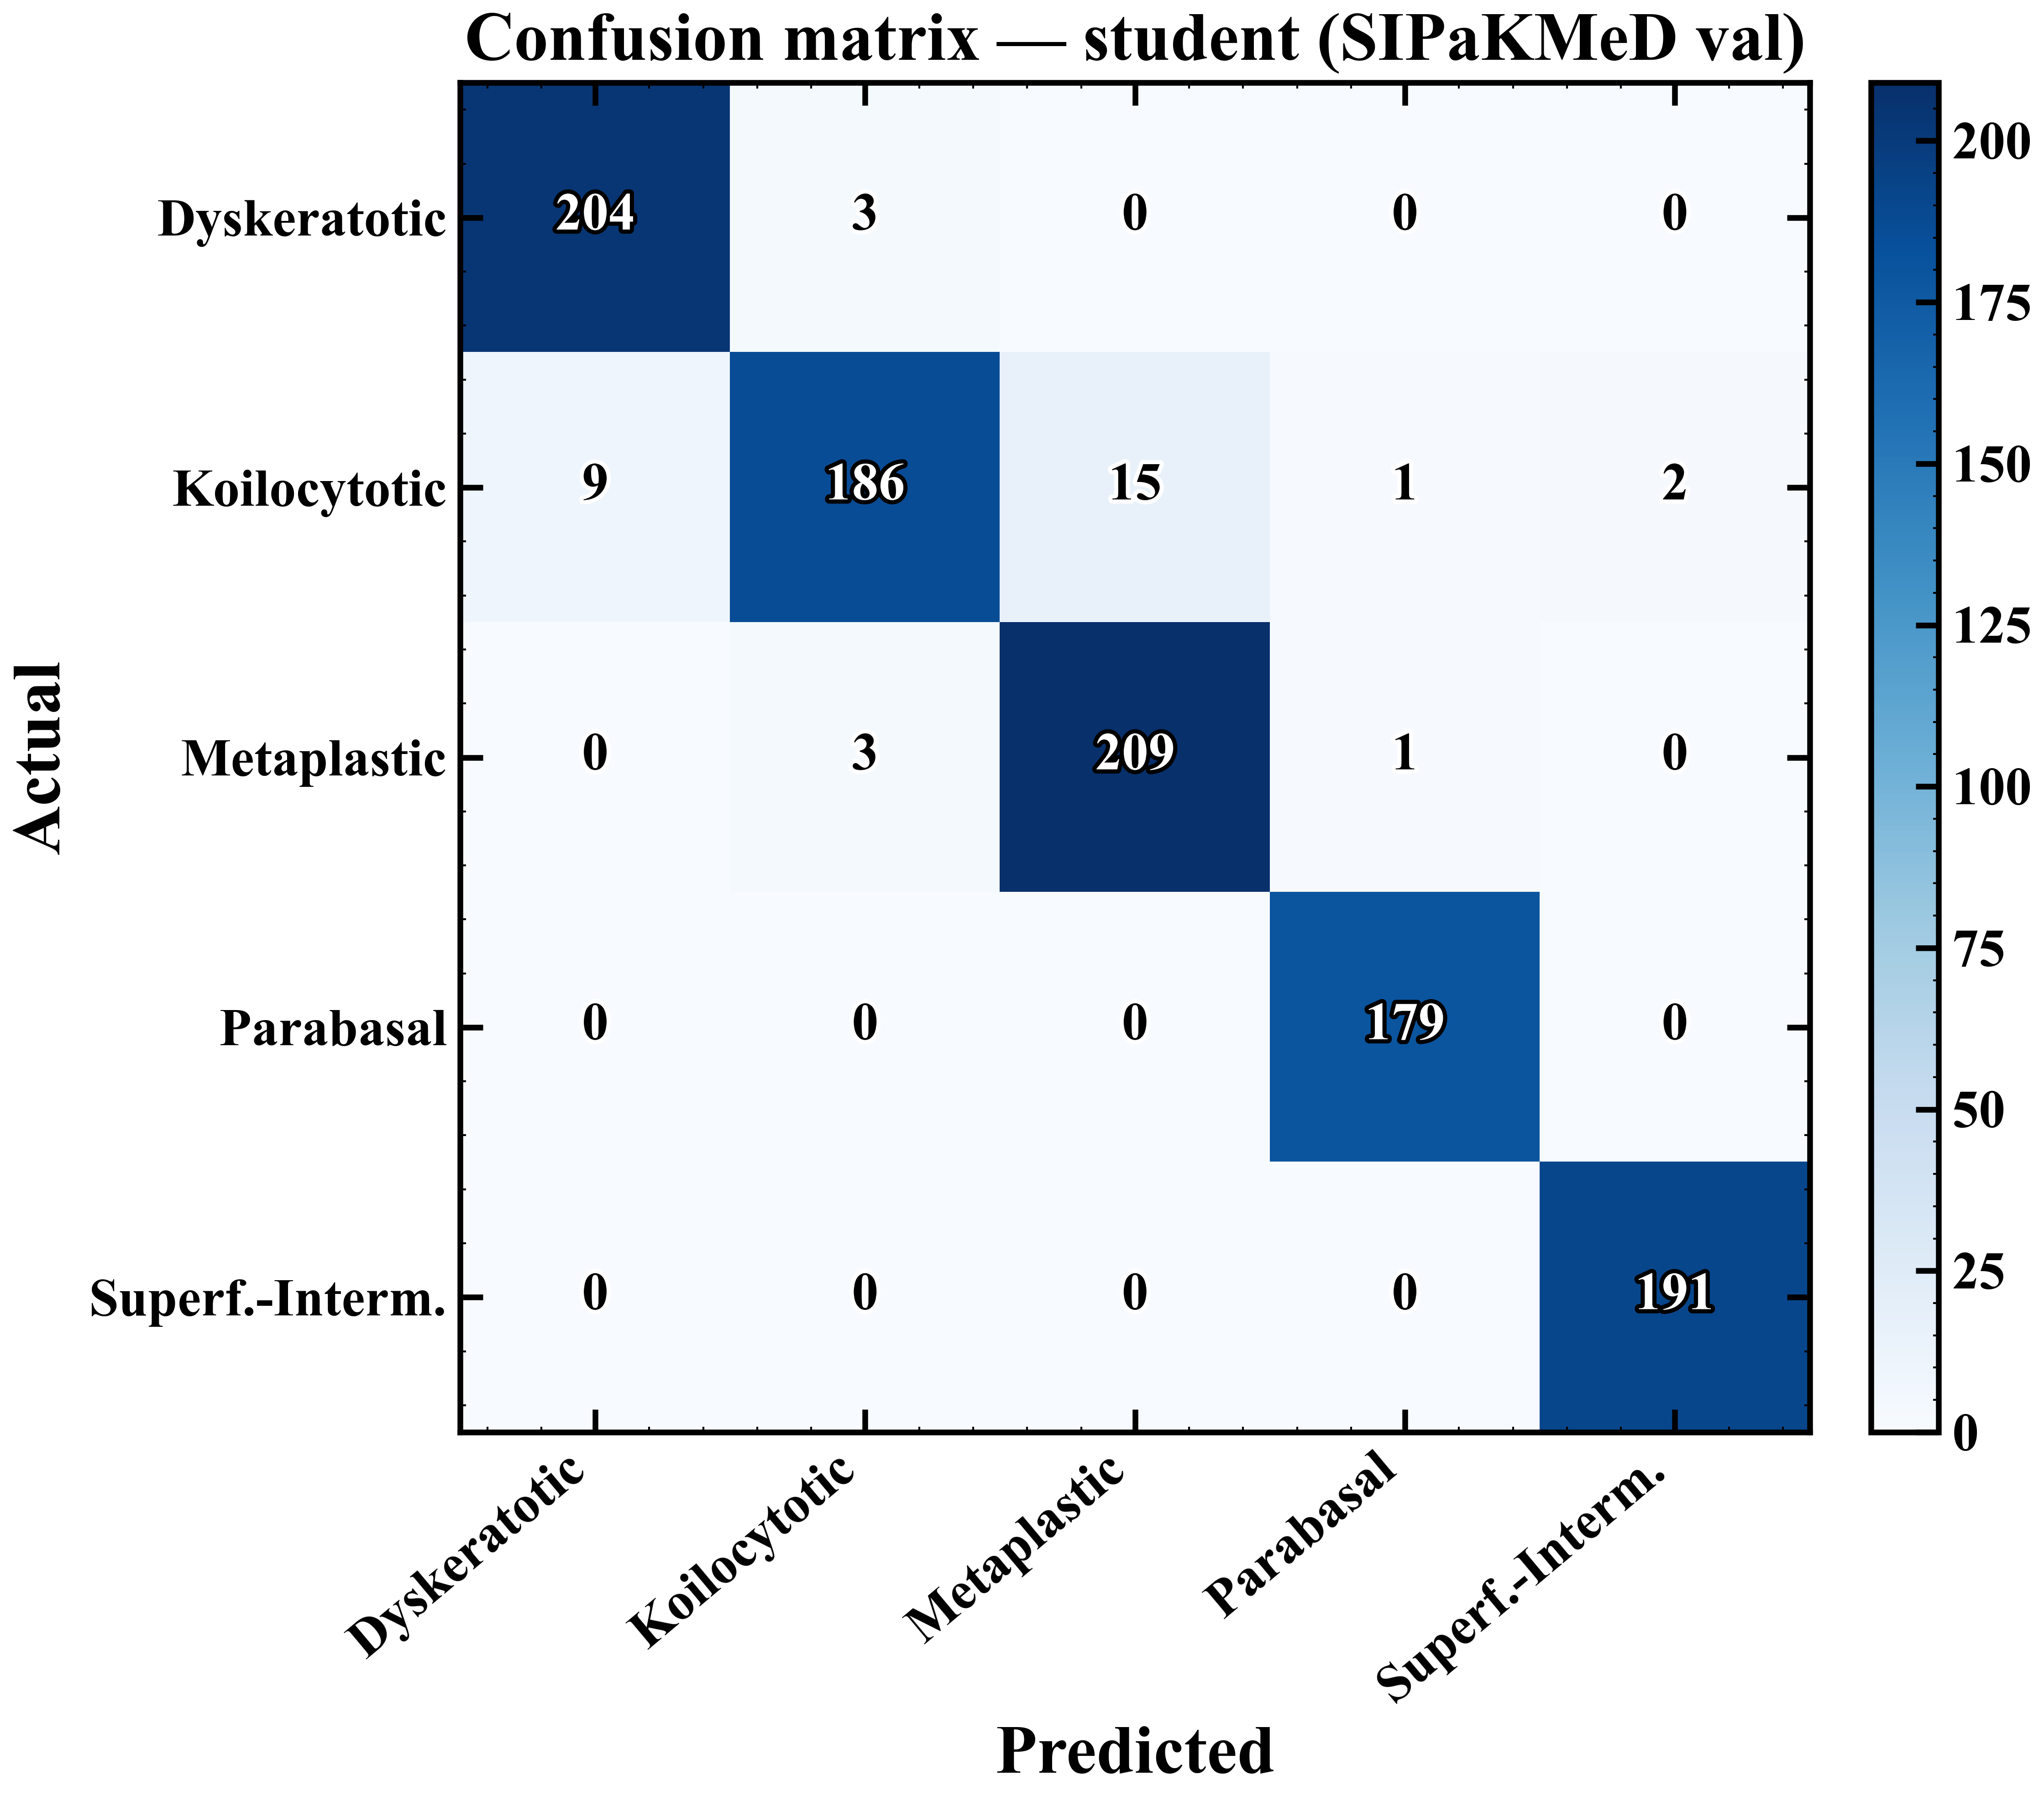
\includegraphics[width=\linewidth]{cm_student.png}
  \caption{\textbf{Five-class confusion matrix (student).} Errors concentrate on Koilocytotic.}
  \label{fig:cm}
\end{figure}

\subsection{Calibration and explainability (answering RQ4, in-distribution)}
Both models are well calibrated in-distribution: ECE $0.013$ (teacher) and $0.015$ (student) on the
five-class problem, falling to $0.008$ for the student on the binary Normal/Abnormal decision, with
reliability bins close to the identity (\cref{fig:reliability}). We carry the binary value forward as
the in-distribution calibration reference, because the cross-dataset evaluation of \cref{sec:analysis}
is binary. Grad-CAM~\cite{selvaraju2017gradcam} over the student's final convolutional block
(\cref{fig:gradcam}) localises the evidence to the nucleus and cell body for one representative
correctly-classified cell per class (confidences $0.97\!-\!1.00$). The attributions are cytologically
plausible---decisions are driven by cell structure, not background artefacts---supporting the
in-distribution half of \textbf{H4}. We stress the standard faithfulness caveat: Grad-CAM shows
\emph{where the model looked}, not that its reasoning is clinically correct. As \cref{sec:analysis}
shows, this in-distribution calibration does \emph{not} survive domain shift.

\begin{figure}[t]
  \centering
  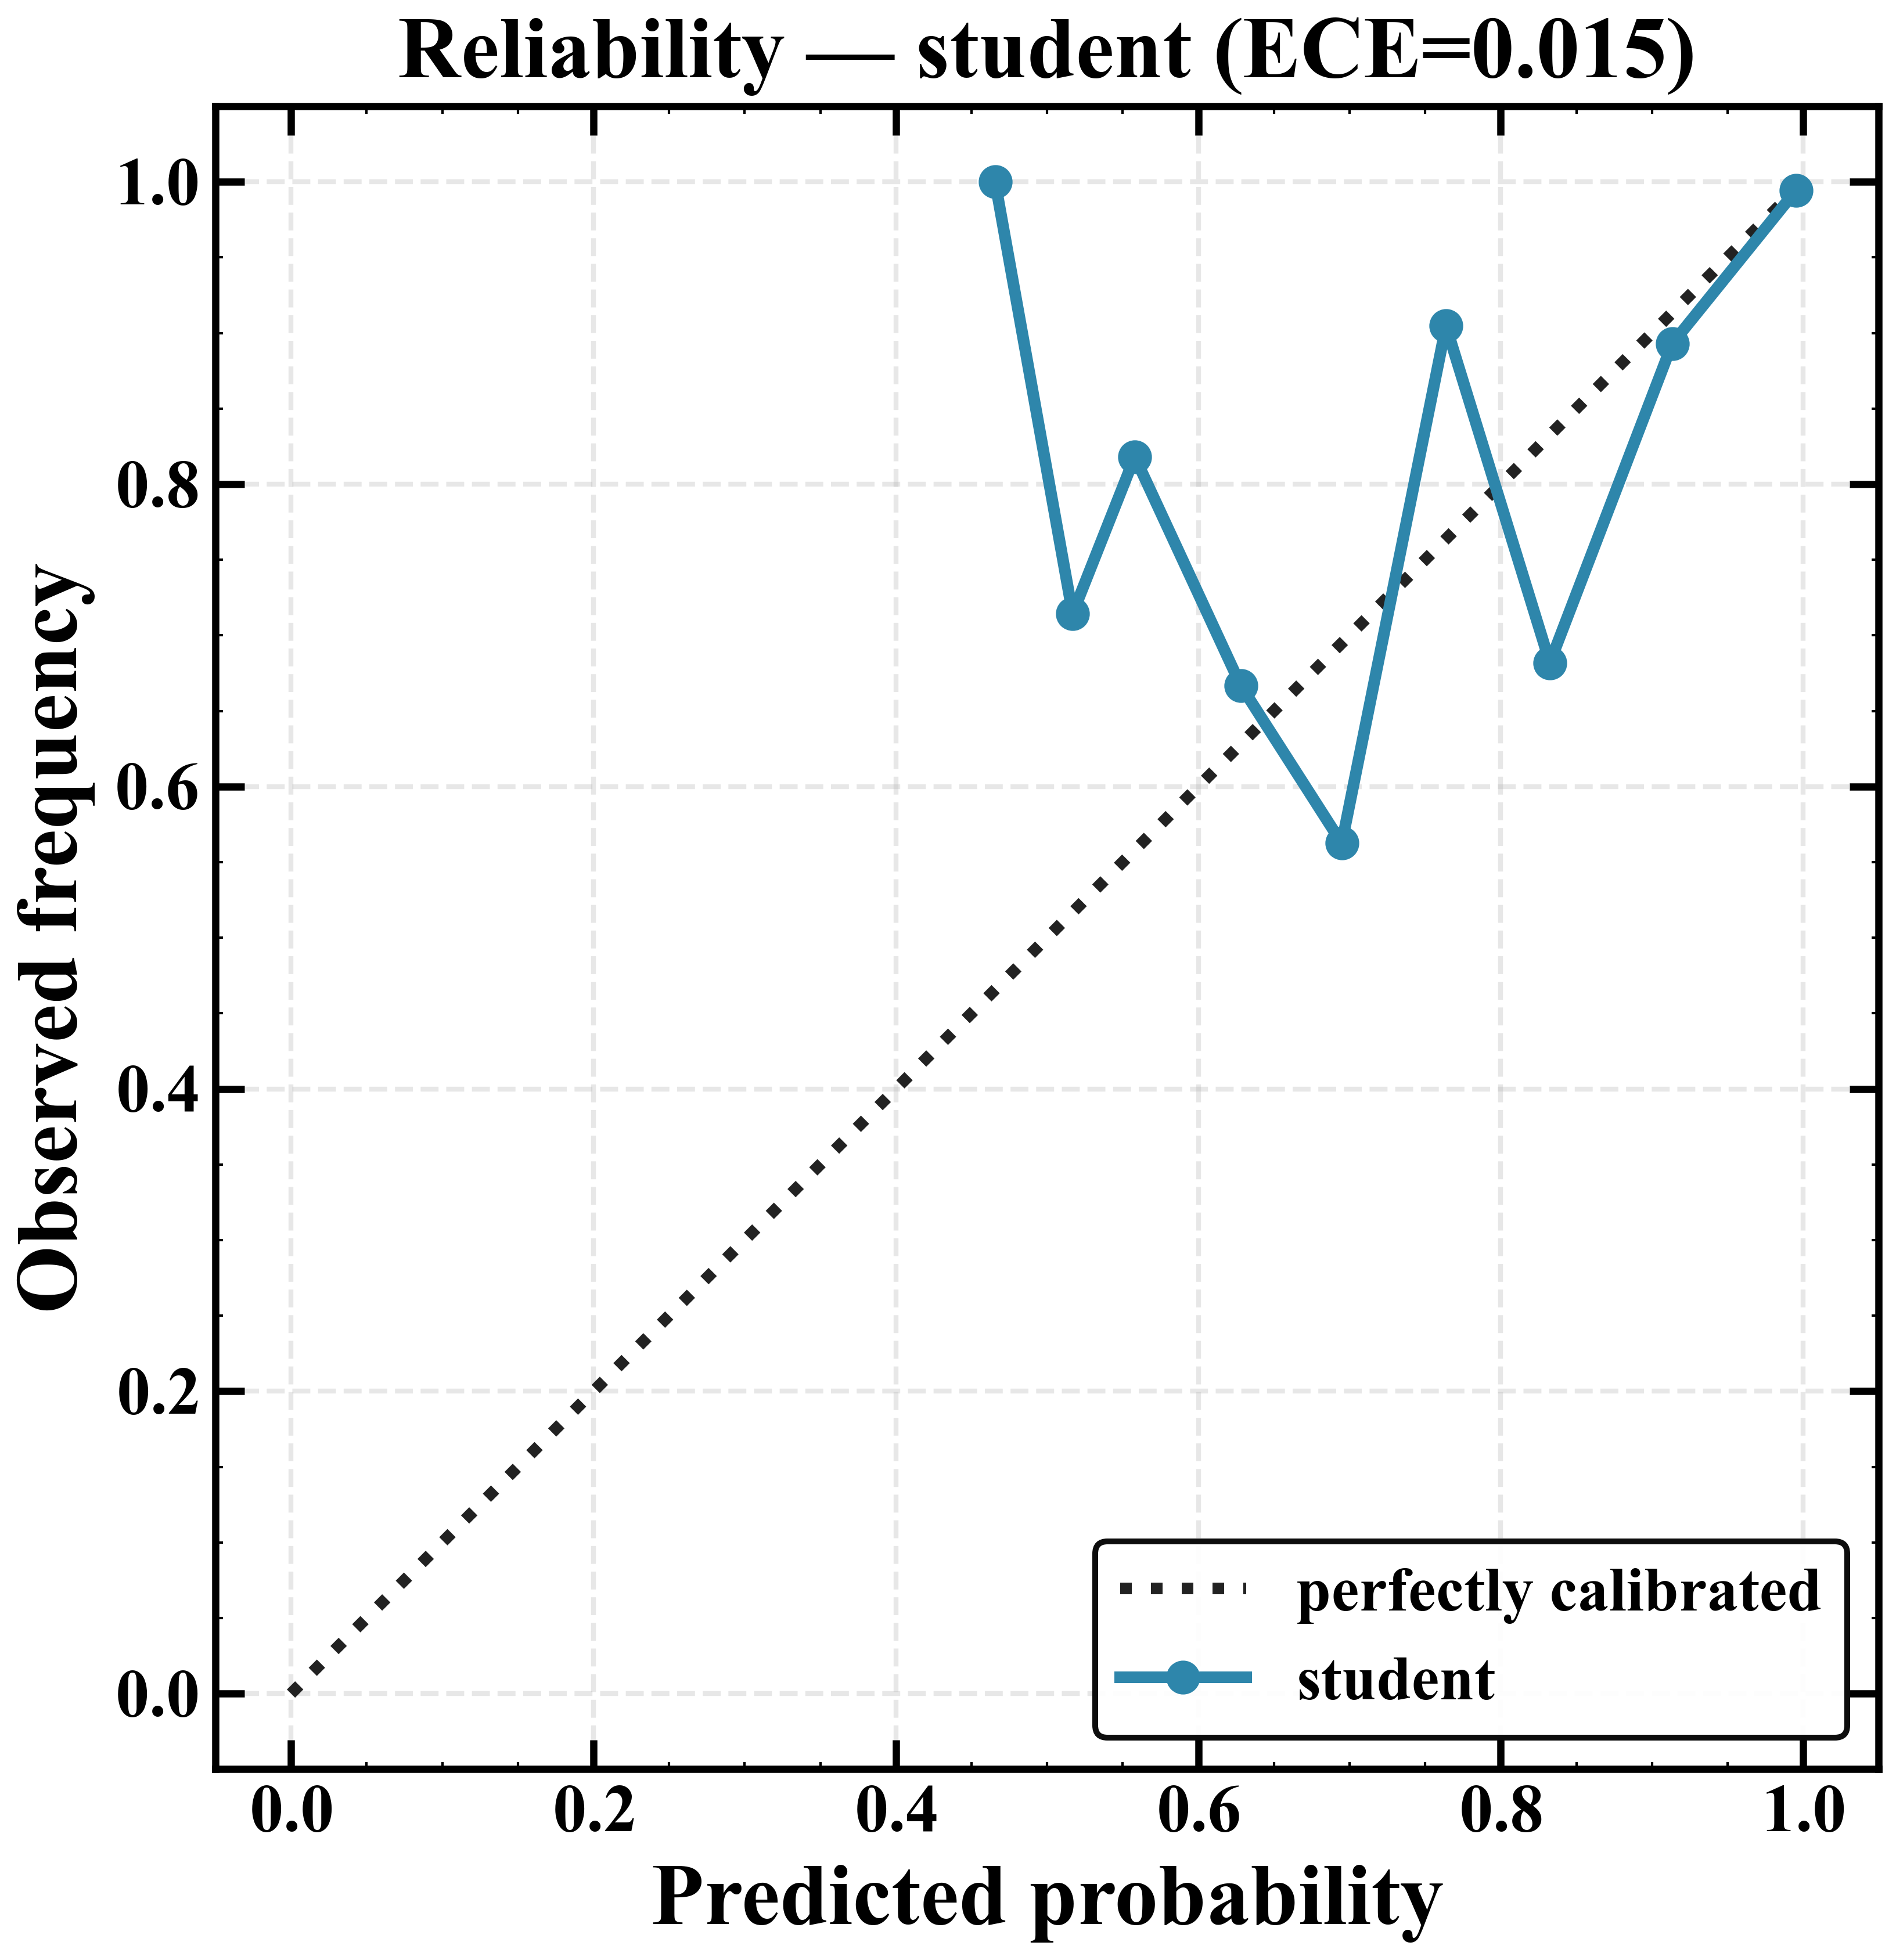
\includegraphics[width=\linewidth]{reliability_student.png}
  \caption{\textbf{Reliability diagram (student).} ECE $0.015$ (five-class): in-distribution
  confidence is well calibrated and sits close to the identity.}
  \label{fig:reliability}
\end{figure}

\begin{figure*}[tb]
  \centering
  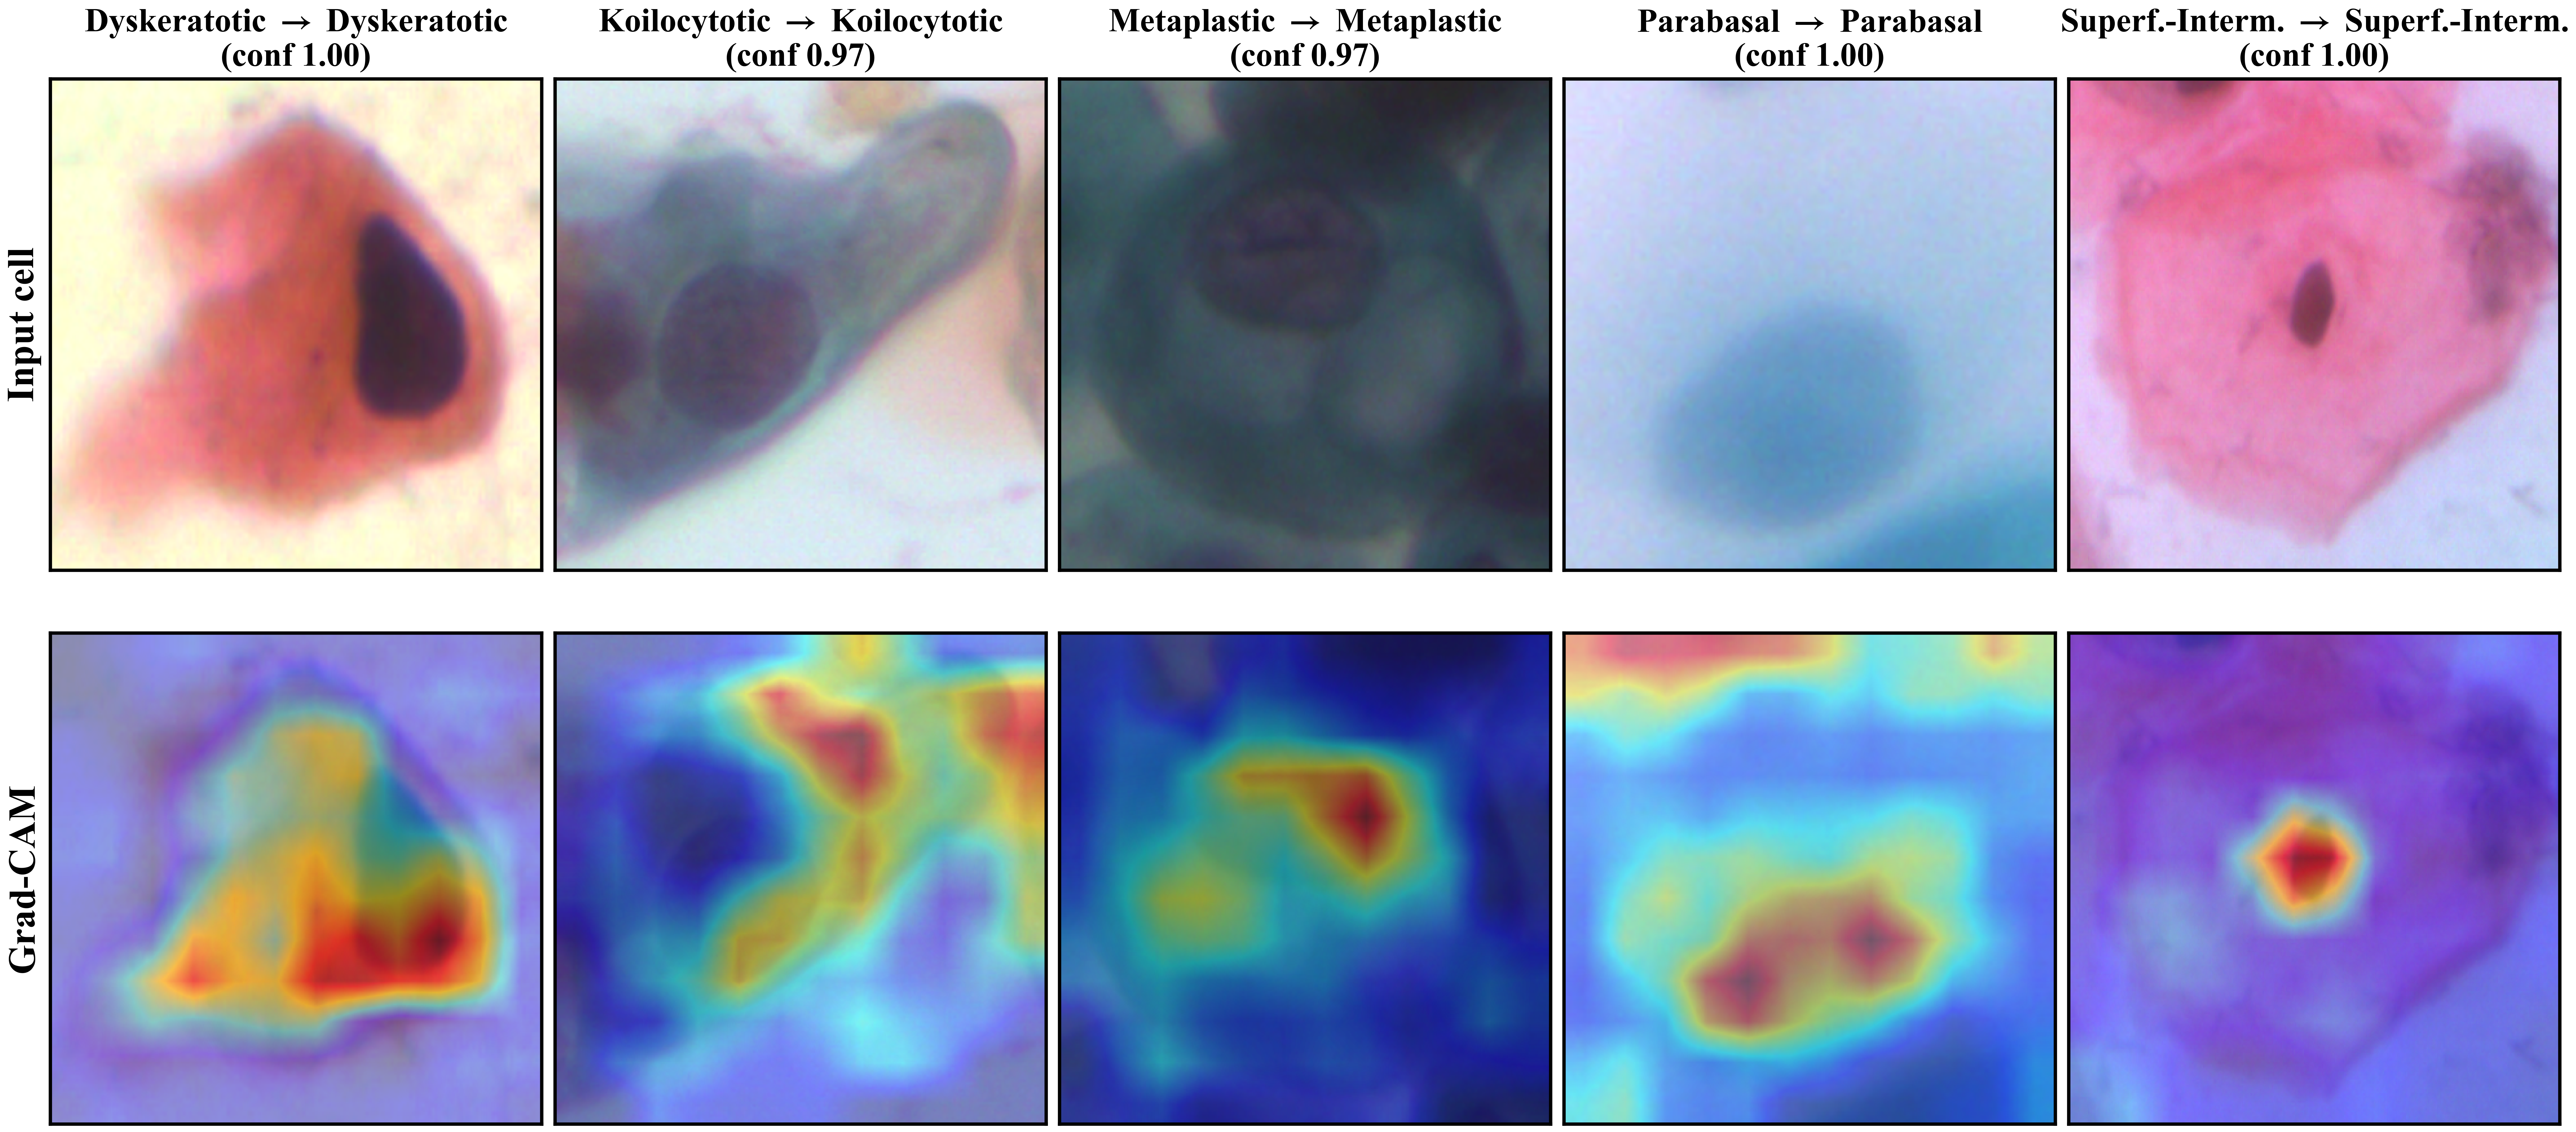
\includegraphics[width=\textwidth]{gradcam_student.png}
  \caption{\textbf{Grad-CAM attributions (student).} One representative cell per class: top row, input
  cell; bottom row, Grad-CAM overlay (true $\rightarrow$ predicted, confidence). Heatmaps localise to
  nuclear/cellular regions; all five sample cells are correctly classified at confidence
  $0.97\!-\!1.00$.}
  \label{fig:gradcam}
\end{figure*}

\section{Cross-dataset collapse and its diagnosis}
\label{sec:analysis}

\subsection{The collapse (answering RQ2)}
Evaluated unchanged on the three external sets under the binary alignment of \cref{tab:mapping},
the student's accuracy falls from $0.966$ internally to $0.639$ (\herlev), $0.605$ (\hicervix) and
$0.532$ (\apacc)---a $33$-to-$43$-point drop (\herlev\ $33$, \hicervix\ $36$, \apacc\ $43$) that
\emph{supports} \textbf{H2} (\cref{tab:cross}, \cref{fig:cmcross}). Threshold-free AUROC tells the
same story more cleanly: $0.728$, $0.594$, $0.525$. Two observations sharpen the result. First, on
\herlev\ and \hicervix\ the accuracy at $\tau{=}0.5$ is \emph{below the majority-class baseline}
($0.639\!<\!0.74$; $0.605\!<\!0.621$, the latter only a razor-thin $1.6$-point gap): a model that
always predicted the majority class would score at least as well. Second, the error structure differs
by dataset---the model over-predicts \emph{abnormal} on \apacc\ (specificity $0.417$) and
\emph{normal} on \hicervix\ (sensitivity $0.386$, missing most abnormal cells). A single global
threshold is clearly mis-placed for each domain.

\begin{table*}[tb]
\caption{\textbf{Cross-dataset binary results (student).} Internal \sipakmed\ accuracy is $0.966$.
ECE is the binary expected calibration error ($15$ bins; in-distribution binary ECE is $0.008$);
$\Delta P$ is the separation between mean $\pabn$ on true-abnormal vs.\ true-normal cells (positive
$=$ correct ordering); ``Maj.'' is the majority-class baseline. At $\tau{=}0.5$, accuracy falls
\emph{below} the majority baseline for \herlev\ and \hicervix\ despite AUROC$>0.5$, and ECE is
$27\!-\!41\times$ the internal value.}
\label{tab:cross}
\centering\small
\begin{tabular}{@{}lccccccccc@{}}
\toprule
Dataset & $n$ & Acc & Bal.\ acc & Sens & Spec & AUROC & ECE & $\Delta P$ & Maj. \\
\midrule
\herlev   & 917  & 0.639 & 0.651 & 0.625 & 0.678 & \best{0.728} & 0.256 & $+0.284$ & 0.74 \\
\hicervix & 4823 & 0.605 & 0.562 & 0.386 & 0.738 & 0.594 & 0.219 & $+0.112$ & 0.62 \\
\apacc    & 1125 & 0.532 & 0.535 & 0.654 & 0.417 & 0.525 & 0.328 & $+0.045$ & 0.51 \\
\midrule
\multicolumn{10}{@{}l}{\footnotesize Internal \sipakmed: Acc $0.966$, binary ECE $0.008$. \quad Higher ECE $=$ worse calibration.}\\
\bottomrule
\end{tabular}
\end{table*}

\begin{figure*}[tb]
  \centering
  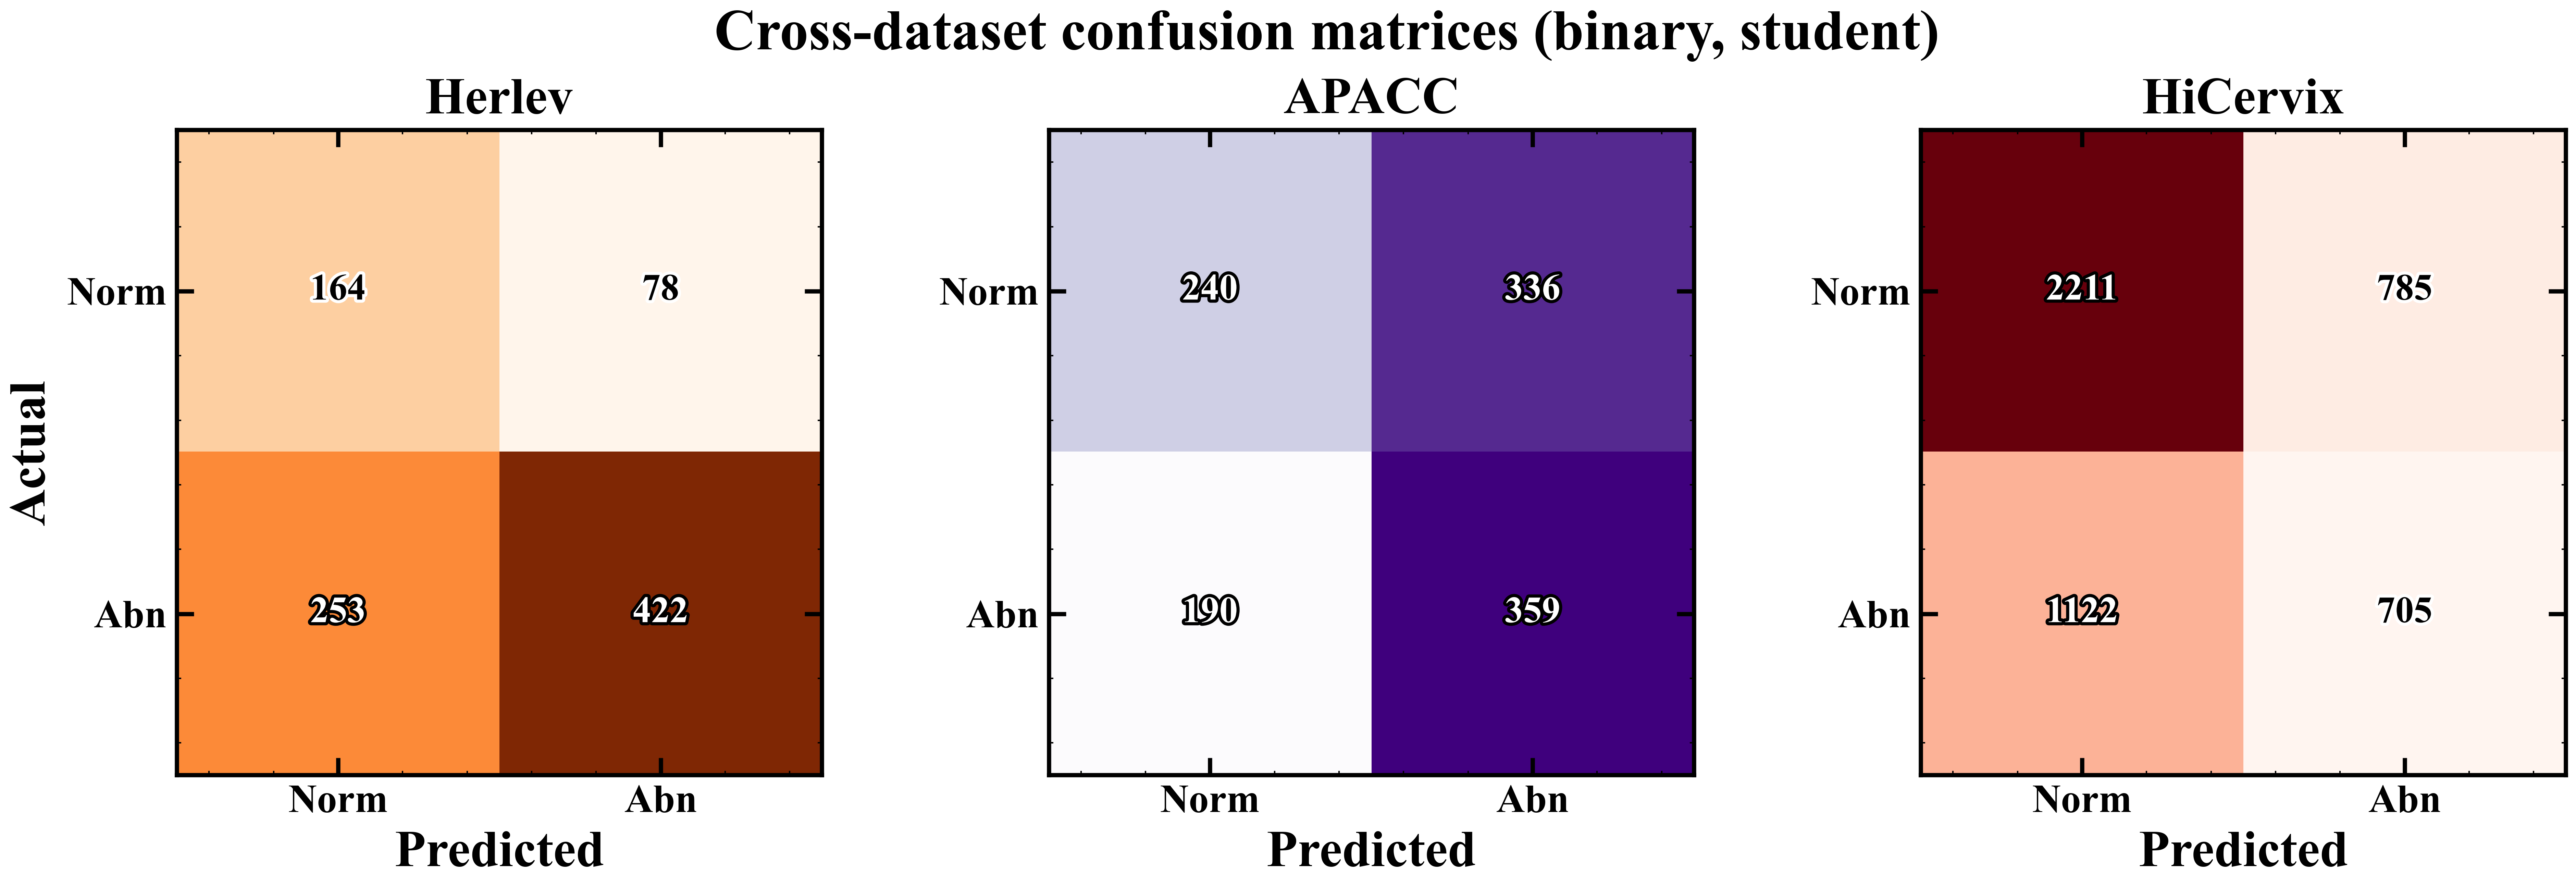
\includegraphics[width=\textwidth]{cm_cross_combined.png}
  \caption{\textbf{Cross-dataset confusion matrices (binary, student).} The model over-predicts
  \emph{abnormal} on \apacc\ (low specificity) and \emph{normal} on \hicervix\ (low sensitivity).}
  \label{fig:cmcross}
\end{figure*}

\subsection{It is not a labelling artefact (answering RQ3)}
The decisive question is whether this collapse is an artefact of our binary crosswalk. It is not. If
the mapping were flipped or mis-defined, the decision score $\pabn$ would rank abnormal cells
\emph{below} normal ones and AUROC would fall \emph{below} $0.5$. The opposite holds in every dataset:
the class-conditional separation $\Delta P=\overline{\pabn}_{\text{abn}}-\overline{\pabn}_{\text{norm}}$
is \emph{positive everywhere} ($+0.284$ \herlev, $+0.112$ \hicervix, $+0.045$ \apacc; \cref{fig:sep},
\cref{tab:cross}) and every AUROC exceeds chance. The score is correctly oriented---the model knows,
weakly, which cells are abnormal---so the labels are not the problem. We additionally audited each
per-dataset mapper against the native taxonomies (\cref{tab:mapping}); the stricter \herlev-columnar
variant shifts the headline by $<\!1$ point. \textbf{H3 is supported}: the failure is genuine, not an
alignment artefact.

\begin{figure*}[tb]
  \centering
  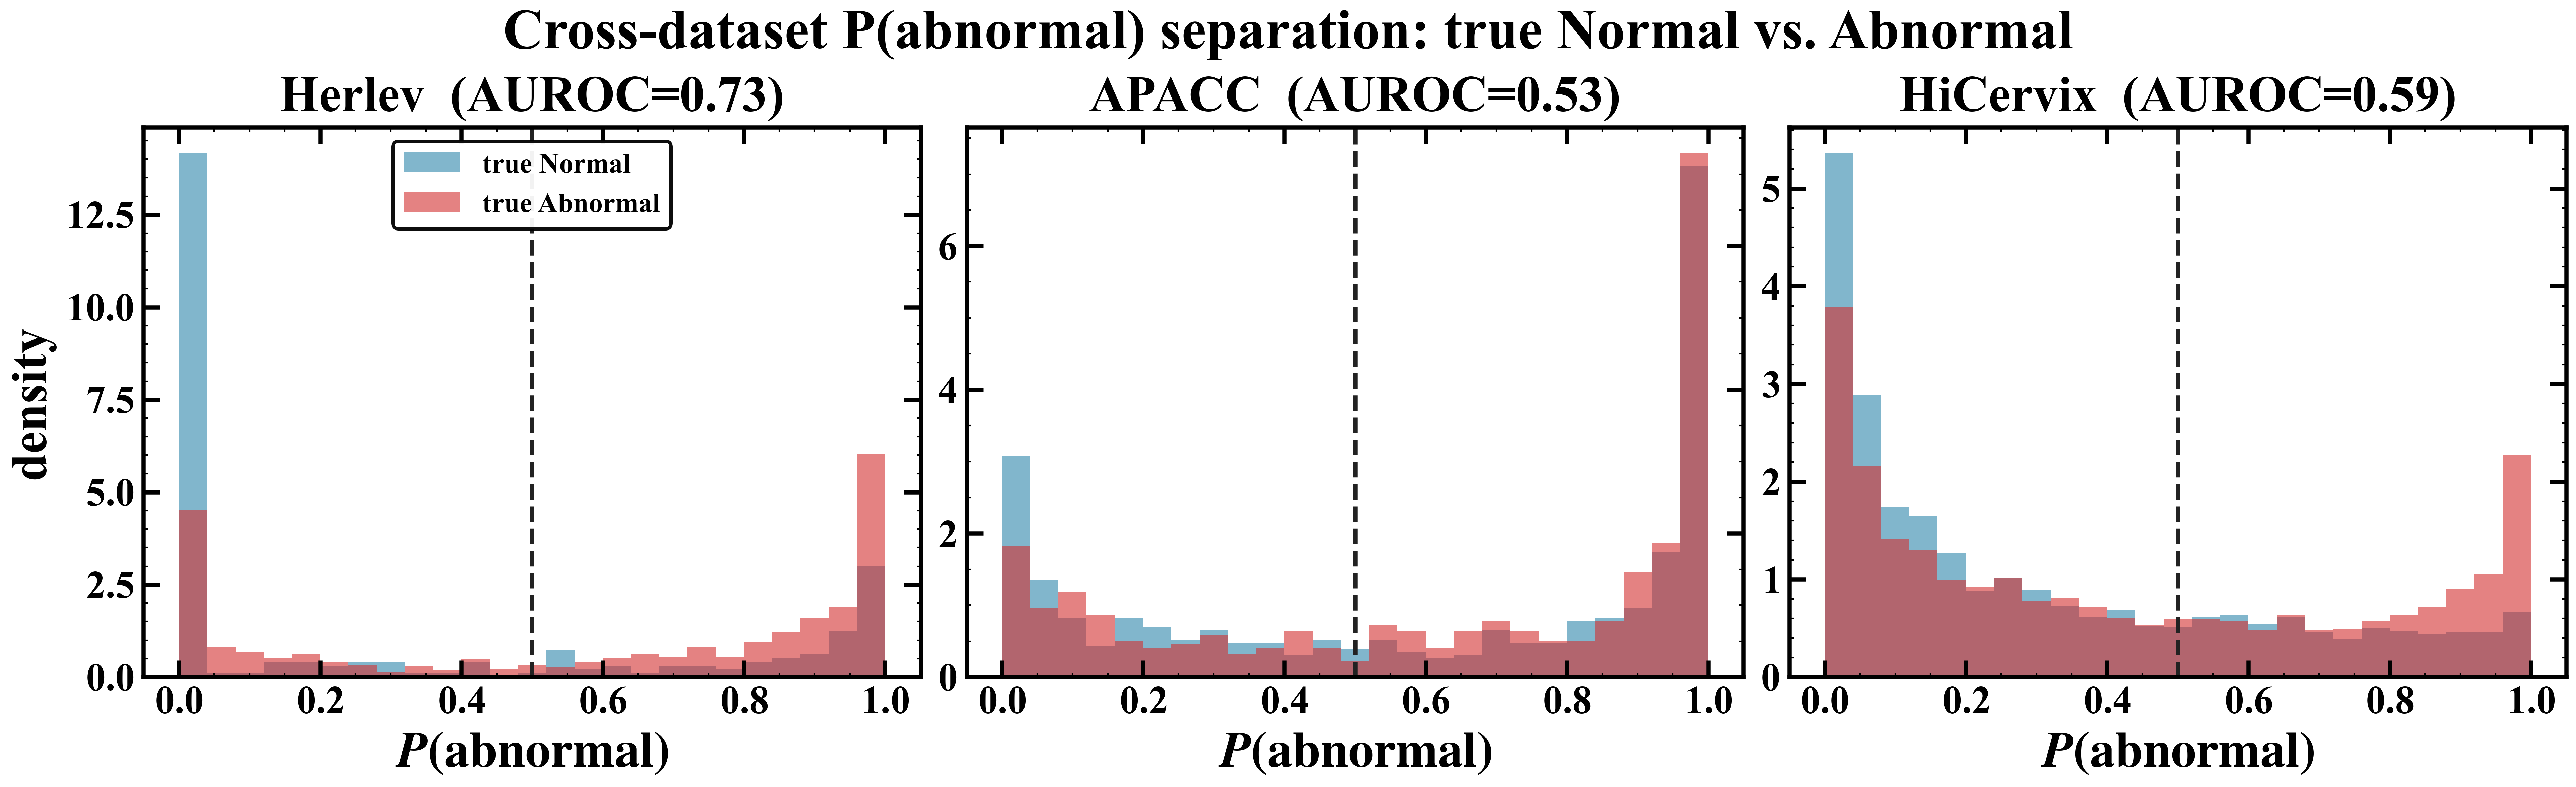
\includegraphics[width=\textwidth]{cross_separation.png}
  \caption{\textbf{$\pabn$ separation.} Distribution of the decision score for true-normal (blue) vs.\
  true-abnormal (red) cells. Separation is clear on \herlev\ (AUROC $0.73$), weak on \hicervix\
  ($0.59$) and essentially absent on \apacc\ ($0.53$). The dashed line is $\tau{=}0.5$; a flipped label
  map would swap the colours and push AUROC below $0.5$.}
  \label{fig:sep}
\end{figure*}

\subsection{What actually breaks}
Three mechanisms, jointly, explain the numbers.

\noindent\textbf{(1) Operating-point miscalibration that does not transfer.} The in-distribution
confidence is well calibrated (binary ECE $0.008$), but this property is \emph{domain-local}: external
binary ECE balloons to $0.256$ (\herlev), $0.219$ (\hicervix) and $0.328$ (\apacc)---a
$27\!-\!41\times$ increase over the internal value (\cref{tab:cross}). The $\pabn$ distribution shifts
wholesale per domain---mean $\pabn$ is $0.61$ on \apacc\ (vs.\ a base abnormal rate of $0.49$, hence
over-calling abnormal) and $0.35$ on \hicervix\ (vs.\ $0.38$, hence under-calling)---so the fixed
$\tau{=}0.5$ lands in the wrong place and discards the ranking signal that AUROC shows is present.
This is exactly why accuracy can fall \emph{below} the majority baseline while AUROC stays above
chance. Quantifying the gap, a per-dataset \emph{oracle} threshold (chosen on the test set, reported
only to bound the calibration loss) recovers accuracy to $0.75$ (\herlev, $\tau{=}0.05$) and $0.65$
(\hicervix, $\tau{=}0.85$)---but not \apacc\ ($0.53$), which has no signal to recover. The
non-transfer of calibration is the cross-dataset half of \textbf{H4}.

\noindent\textbf{(2) Signal degrades with slide-preparation distance.} The retained AUROC is ordered
by how far each dataset's preparation sits from \sipakmed's conventional smear:
\herlev\ (conventional) $0.73$ $>$ \hicervix\ (liquid-based) $0.59$ $>$ \apacc\ (auto-segmented noisy
crops) $0.53\!\approx\!$ chance. The model has, in effect, learned features entangled with the
preparation pipeline---a cytology instance of shortcut learning~\cite{geirhos2020shortcut}---and the
discriminative signal erodes monotonically as that pipeline diverges.

\noindent\textbf{(3) The internal number is itself optimistic.} The $0.966$ is measured on a random
per-cell split, which places cells from the \emph{same} field-of-view into both train and validation;
those cells share staining, focus and debris, so the validation estimate is inflated by leakage. A
leakage-safe, cluster-grouped split (no field-of-view shared across partitions) would lower it,
widening the true internal-to-external gap beyond the $33\!-\!43$ points measured here. The honest
headline is therefore worse than even \cref{tab:cross} suggests.

\section{Discussion}
\label{sec:discussion}

\noindent\textbf{The distillation paradox.} The student is \emph{smaller and stronger} than its
teacher in-distribution ($0.966$ vs.\ $0.943$, every metric; \cref{tab:indist}) yet \emph{no more
robust} out-of-distribution (both collapse under the same domain shift). Distillation here acts as a
regulariser---the temperature-softened teacher targets smooth the student's decision surface on the
training distribution---but it transfers the teacher's \emph{inductive biases}, including its reliance
on preparation-entangled features. Compression bought accuracy and efficiency, not generalisation. A
practitioner who reads only the in-distribution number would deploy a model that is wrong more often
than a constant predictor on two of three external sites.

\noindent\textbf{Why a single in-distribution metric misleads.} Three numbers that look reassuring in
isolation each hide the failure: accuracy ($0.966$) is inflated by field-of-view leakage; ECE
(binary $0.008$ in-distribution) is domain-local and balloons to $0.22$--$0.33$ under shift; and AUROC
stays $>0.5$ externally even where
\emph{accuracy is below the majority baseline}, so a threshold-free metric alone would also mislead in
the opposite direction. The collapse is only visible when these are read \emph{together} and
\emph{per-domain}---which is the audit protocol we advocate.

\noindent\textbf{What would actually help.} Our diagnosis points to specific, testable remedies rather
than generic ``train on more data''. (i) \textbf{Per-domain threshold calibration:} the oracle analysis
shows a single re-tuned $\tau$ recovers $0.75$/$0.65$ on \herlev/\hicervix, so even a handful of
labelled target cells would substantially help where ranking signal survives. (ii)
\textbf{Preparation-invariant features:} stain normalisation~\cite{macenko2009stain} and
preparation-aware augmentation to break the shortcut~\cite{geirhos2020shortcut}. (iii)
\textbf{Leakage-safe evaluation:} cluster-grouped splits so the internal number is honest from the
start. (iv) \textbf{Report the floor:} always print the majority baseline next to accuracy, so a
below-baseline operating point cannot hide.

\noindent\textbf{Limitations.} We audit one architecture family (EfficientNet) and one training
source (\sipakmed); the \emph{magnitude} of collapse may differ for other backbones, though the
mechanism---non-transferable operating point plus preparation shortcut---is general. The oracle
thresholds are computed on the test set and are an \emph{upper bound} on what calibration could
recover, not a deployable result. The binary crosswalk, while deterministic and documented, discards
glandular and out-of-scope cells; we report that excluded fraction but do not evaluate on them. Grad-CAM
is a localisation, not a faithfulness, guarantee. None of these qualifies the central finding: strong
internal numbers do not imply cross-site readiness, and the gap is measurable and mechanistically
explainable.

\section{Conclusion}
\label{sec:conclusion}

We audited a knowledge-distilled cervical-cytology classifier the way it would be \emph{used}, not the
way it is usually \emph{reported}: we froze it after strong in-distribution training and measured it on
three external Pap datasets spanning the slide-preparation axis. The result is a clean cautionary tale.
In-distribution the distilled B0 student is excellent and \emph{beats its own B4 teacher}
(accuracy $0.966$, AUROC $0.998$, ECE $0.015$) at a quarter of the parameters. Pushed across datasets,
the same weights collapse to $0.639$/$0.605$/$0.532$ accuracy and $0.728$/$0.594$/$0.525$ AUROC---at
two sites below what a constant majority predictor would score.

Our central contribution is the \emph{diagnosis}, not the collapse. We show it is \emph{not} a labelling
artefact---the $\pabn$ score is correctly oriented everywhere ($\Delta P>0$, AUROC$>0.5$)---but the
joint product of an operating point that does not transfer (in-distribution calibration is domain-local:
binary ECE rises from $0.008$ to $0.22$--$0.33$ across sites) and features entangled with slide
preparation (retained signal falls monotonically with preparation
distance: conventional $>$ liquid-based $>$ auto-segmented). We further show the internal $0.966$ is
itself optimistic under field-of-view leakage, so the true gap is wider still. Each finding is tied to a
falsifiable test and a concrete remedy---per-domain threshold calibration, preparation-invariant
features, leakage-safe splits, and always reporting the majority floor.

The broader lesson generalises past cytology: a single in-distribution metric---accuracy, calibration,
or AUROC alone---can each independently hide a model that is unfit for cross-site deployment. Honest
medical-imaging evaluation must be multi-metric, per-domain, leakage-aware, and reported against the
majority baseline. We release the full audit protocol and per-dataset breakdowns
(\cref{sec:appA}) to make such reporting routine.


\appendix
\section{Reproducibility and protocol details}
\label{sec:appA}

\noindent\textbf{Environment.} PyTorch $2.11$ (CUDA $12.8$), single NVIDIA RTX $5060$\,Ti ($16$\,GB),
BF16 autocast, deterministic seed $42$, \texttt{num\_workers}$=0$. All numbers in this paper are
produced by the frozen checkpoints; we report measured values only and do not extrapolate.

\noindent\textbf{Models and optimisation.} EfficientNet-B4 teacher ($18.5$\,M) and B0 student
($4.67$\,M), ImageNet-pretrained, custom head $\mathrm{BN}\!\to\!\mathrm{Linear}(512)\!\to\!
\mathrm{ReLU}\!\to\!\mathrm{Dropout}\!\to\!\mathrm{Linear}(5)$. Teacher: Adam, class-weighted CE,
two stages (frozen lr $10^{-3}$ $\le\!30$ ep; fine-tune lr $10^{-5}$ $\le\!50$ ep), ReduceLROnPlateau
on val loss. Student: KD (\cref{eq:kd}, $T{=}4$, $\alpha{=}0.1$), Adam lr $5\!\times\!10^{-5}$,
$\le\!40$ ep, early-stopped on val accuracy. Input $380\!\times\!380$, ImageNet normalisation; train
augmentation = flips $+$ rotation $\pm72^{\circ}$ $+$ affine scale $0.9\!-\!1.1$; eval = resize $+$
normalise only.

\noindent\textbf{Split.} Per-class stratified $80/20$ over the $5{,}015$ \sipakmed\ images
($4{,}012$ train / $1{,}003$ val). We note explicitly (\cref{sec:analysis}) that this random per-cell
split shares field-of-view across partitions and therefore overstates internal accuracy; a
cluster-grouped split is the recommended fix.

\noindent\textbf{Binary decision and metrics.} $\pabn=\softmax(z)_{\text{Koilo}}+\softmax(z)_{\text{Dysk}}$
(\cref{eq:pabn}); predict Abnormal if $\pabn>\tau$, $\tau{=}0.5$. We report accuracy, balanced
accuracy, sensitivity, specificity, threshold-free AUROC, the class-conditional separation
$\Delta P$, ECE ($15$ equal-width bins), and---next to every external accuracy---the majority-class
baseline. Oracle thresholds are swept on the test set and reported only to bound recoverable
calibration loss; they are not a deployable result.

\noindent\textbf{External evaluation counts.} \herlev\ $917$ cells; \apacc\ $1{,}125$ crops (one
zero-byte file removed; \texttt{rubbish}/\texttt{bothcells} excluded); \hicervix\ $4{,}823$ scorable of
$8{,}051$ test cells (\texttt{AGC}/\texttt{microbe} excluded); \herlev\ \texttt{columnar} mapped to Normal
in the legacy crosswalk (stricter exclusion variant moves the headline $<\!1$ point). Excluded
fractions are reported so that dropping unmappable cells cannot silently inflate the binary score.

\noindent\textbf{Explainability.} Grad-CAM~\cite{selvaraju2017gradcam} on the student's final
convolutional block; one representative correctly-classified cell per class
(\cref{fig:gradcam}, confidences $0.97\!-\!1.00$). Attributions are localisation evidence, not a
faithfulness guarantee.


{\small
\bibliographystyle{ieeenat_fullname}
\bibliography{refs}
}

\end{document}
